
\documentclass[12pt]{article}
\usepackage{graphicx}
\usepackage{float}
\usepackage[margin=1in]{geometry}
\usepackage{caption}

\begin{document}

\section{Results} 

% Combined Accuracy Distribution
\subsection{Overall Accuracy Distribution}
\begin{figure}[H]
    \centering
    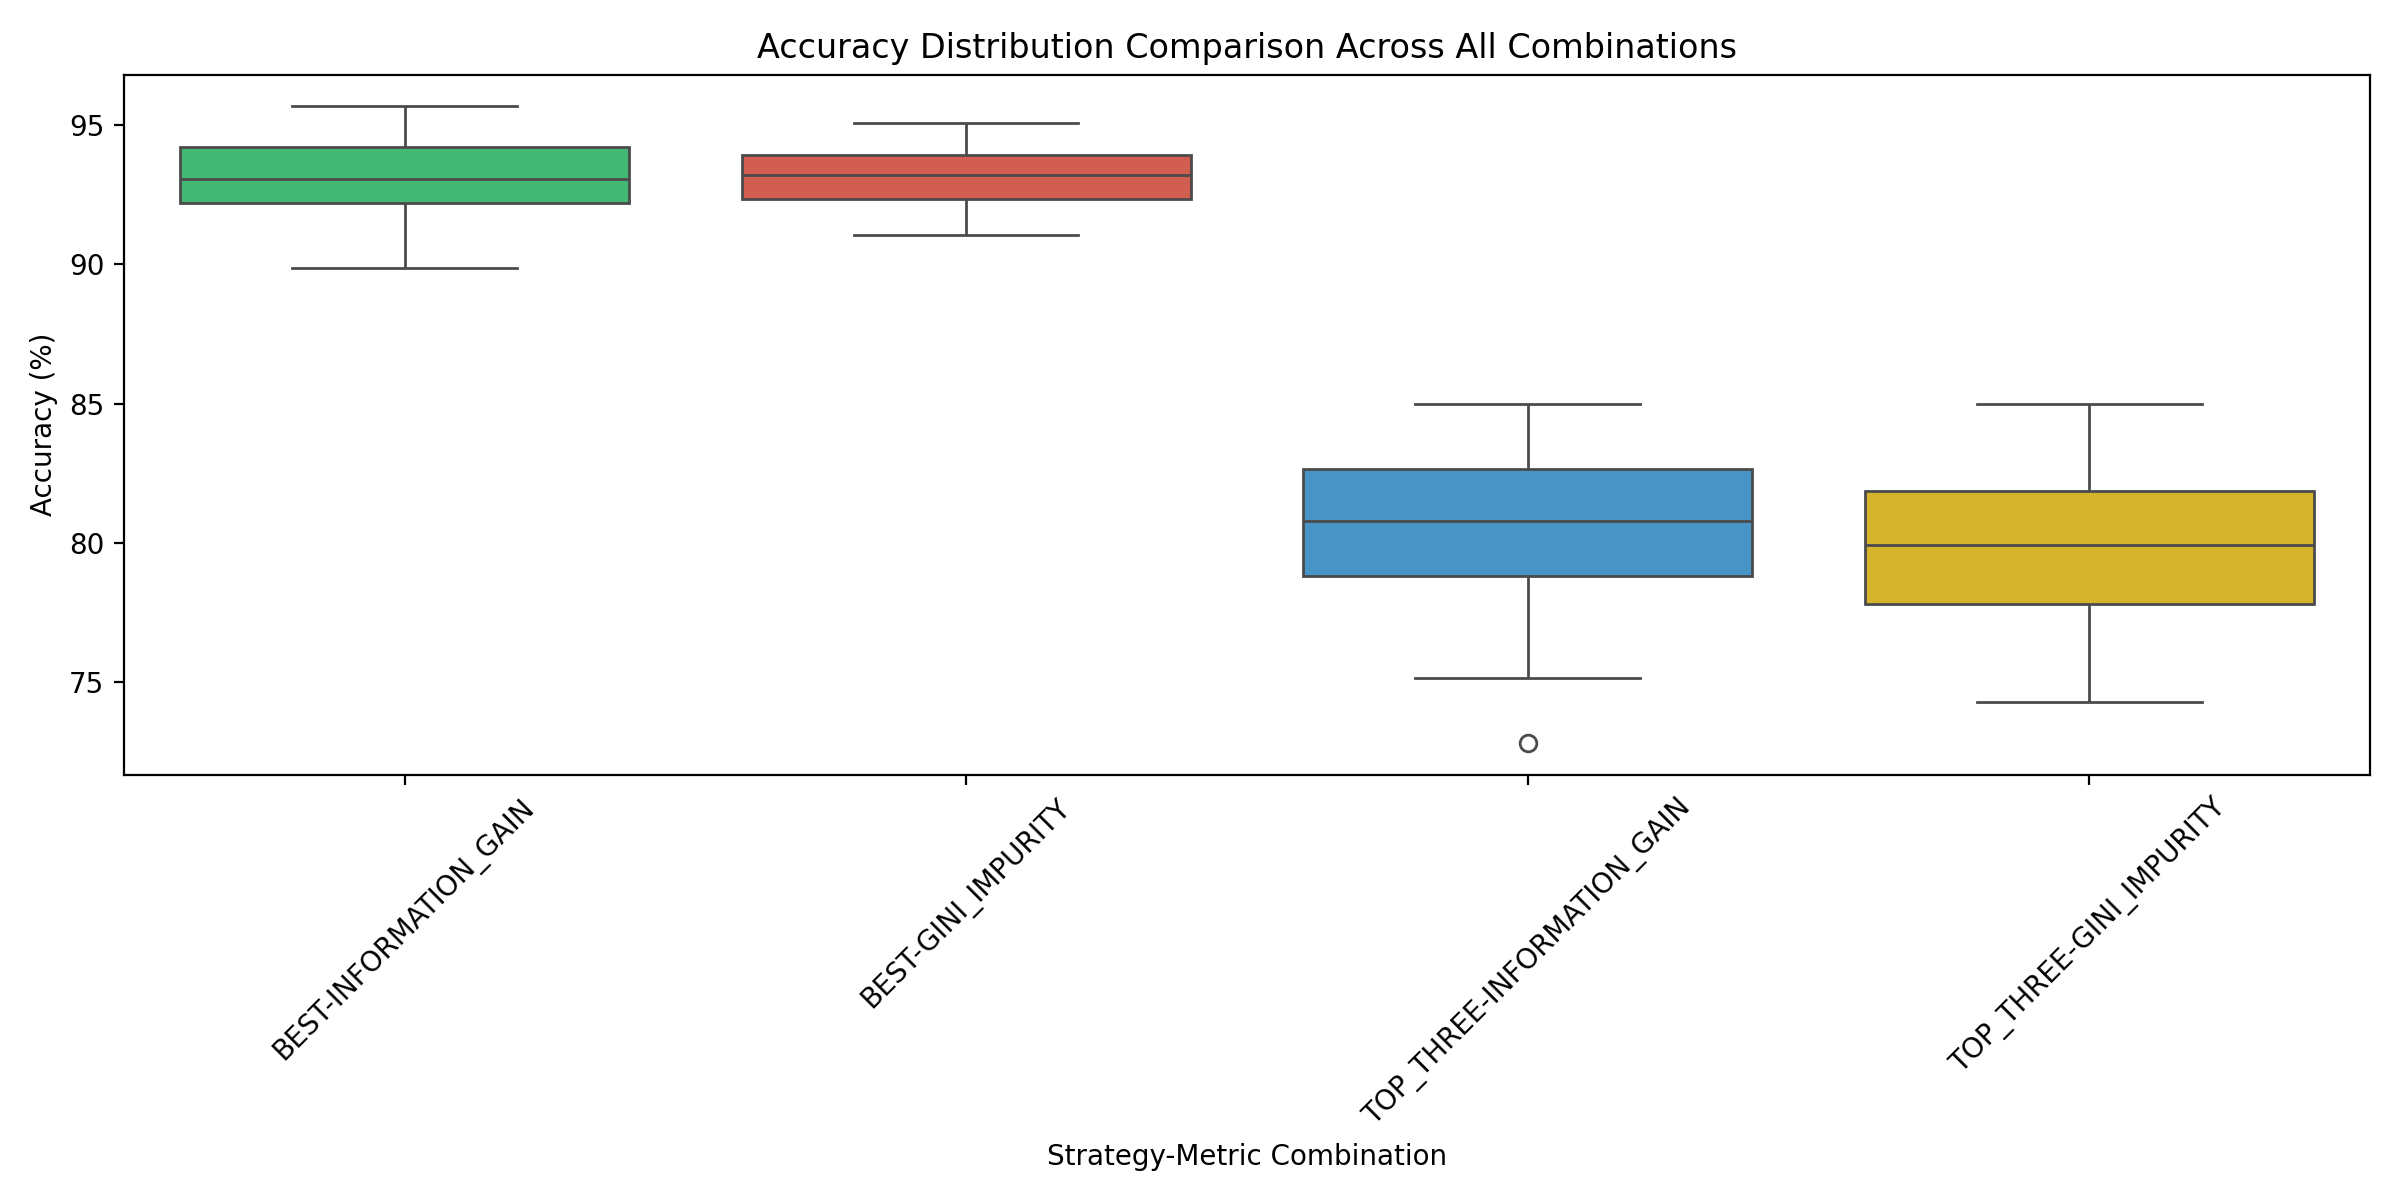
\includegraphics[width=0.9\textwidth]{plots/combined_accuracy_distribution.png}
    \caption{Comparison of accuracy distributions across different strategy and metric combinations.}
    \label{fig:combined-accuracy}
\end{figure}

The above box-whisker plot demonstrates the test-set accuracy of the decision tree built in case of 4 different combinations of selection strategy and evaluation metrics.

It is evident that the accuracy attains its maximum when we take the best attribute while testing at each node and the evaluation metric is set to be the Information Gain. The accuracy, in case of Gini Impurity is also very close to the previous case. However, when we pick one random attribute from the top three, not only does the mean accuracy drop, but also does the accuracy deviate more over several runs, thereby making it less consistent.

\newpage

% Combined Confusion Matrices
\subsection{Classification Performance Analysis}
\begin{figure}[H]
    \centering
    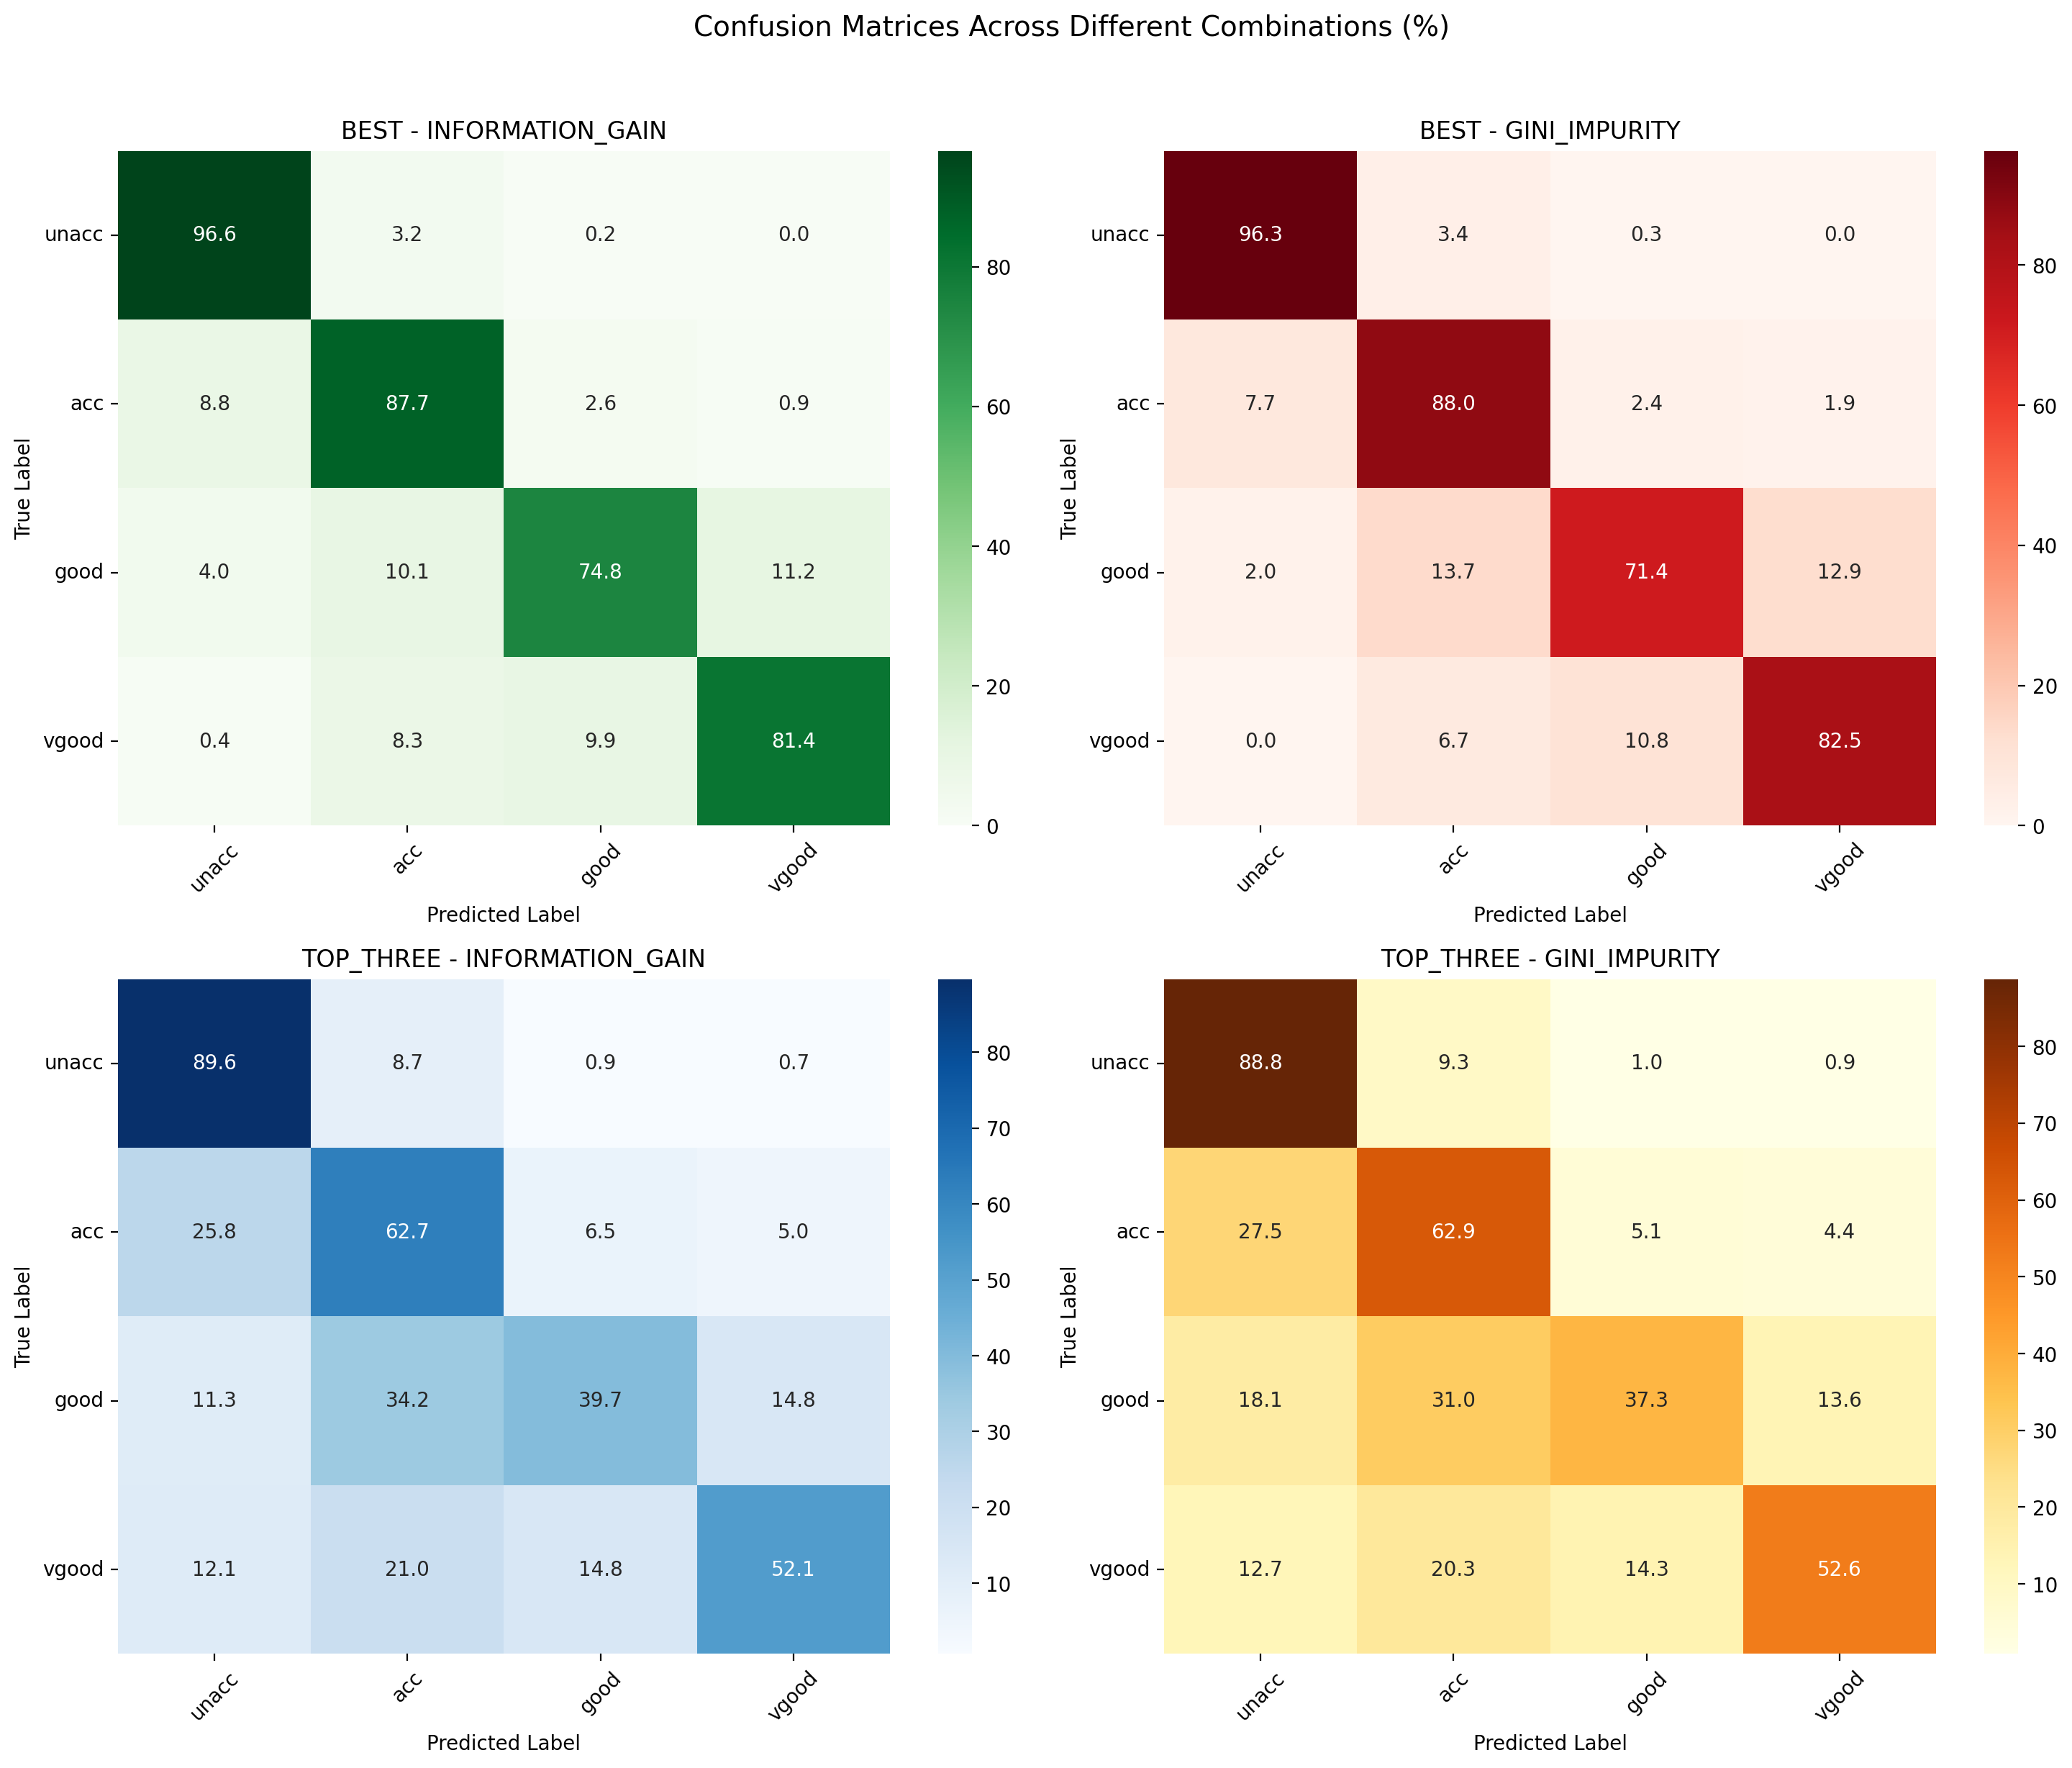
\includegraphics[width=\textwidth]{plots/confusion_matrices_combined.png}
    \caption{Confusion matrices showing classification performance across different strategy-metric combinations. Each subplot uses a different color gradient for better distinction.}
    \label{fig:confusion-matrices}
\end{figure}

The confusion matrices give insights about which class pairs the decision tree often confuse between.

For instance, it often classifies "good" ones as "acc", as can be observed in all of the confusion matrices. And in case of random-choice from three attributes, it also often tends to classify "vgood" classes as "acc" or "good". Also, in case of random picking from top three, the confusion matrix appears more scattered and inconsistencies are higher.

\newpage

% Combined Error Rates
\subsection{Error Rate Analysis}
\begin{figure}[H]
    \centering
    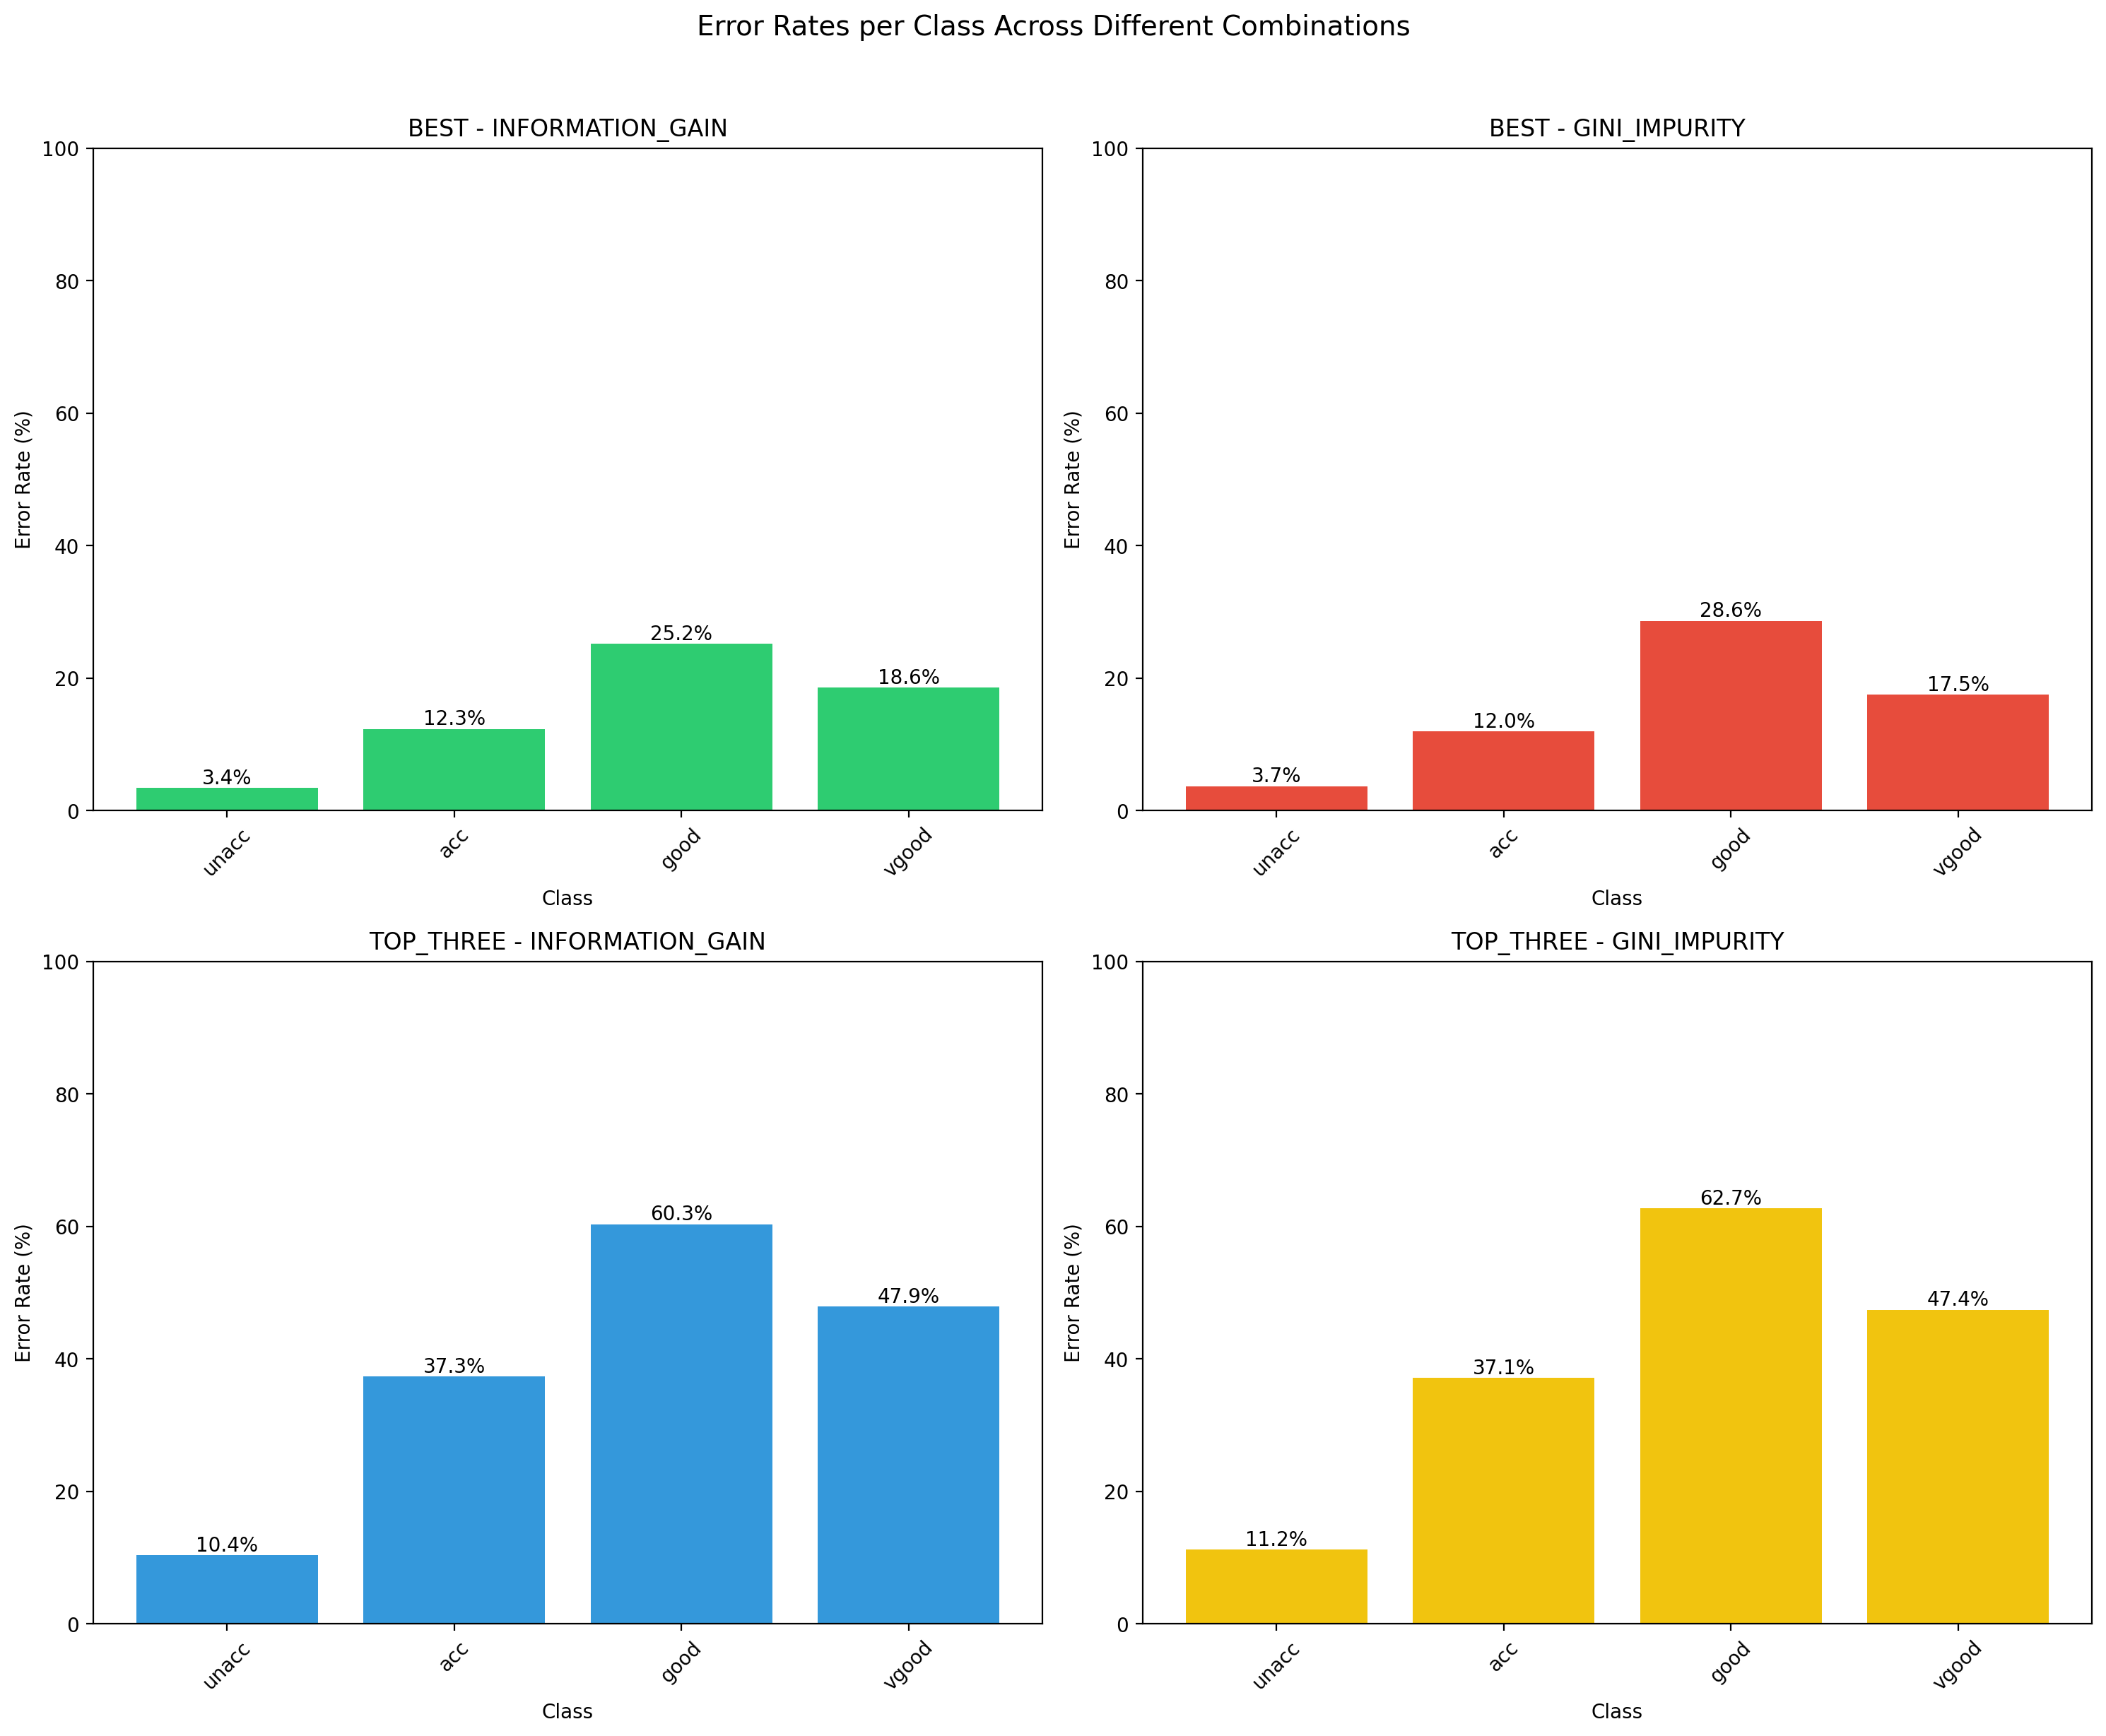
\includegraphics[width=\textwidth]{plots/error_rates_combined.png}
    \caption{Error rates per class across different strategy-metric combinations, showing the misclassification percentages for each category.}
    \label{fig:error-rates}
\end{figure}

These plots show that the decision tree, in almost all cases, classifies "unacc" classes correctly. On the contrary, the maximum error rates are observed in case of "good" class.

\newpage

% Attribute Depths (Individual plots still)
\subsection{Attribute Depth Analysis}
\begin{figure}[H]
    \centering
    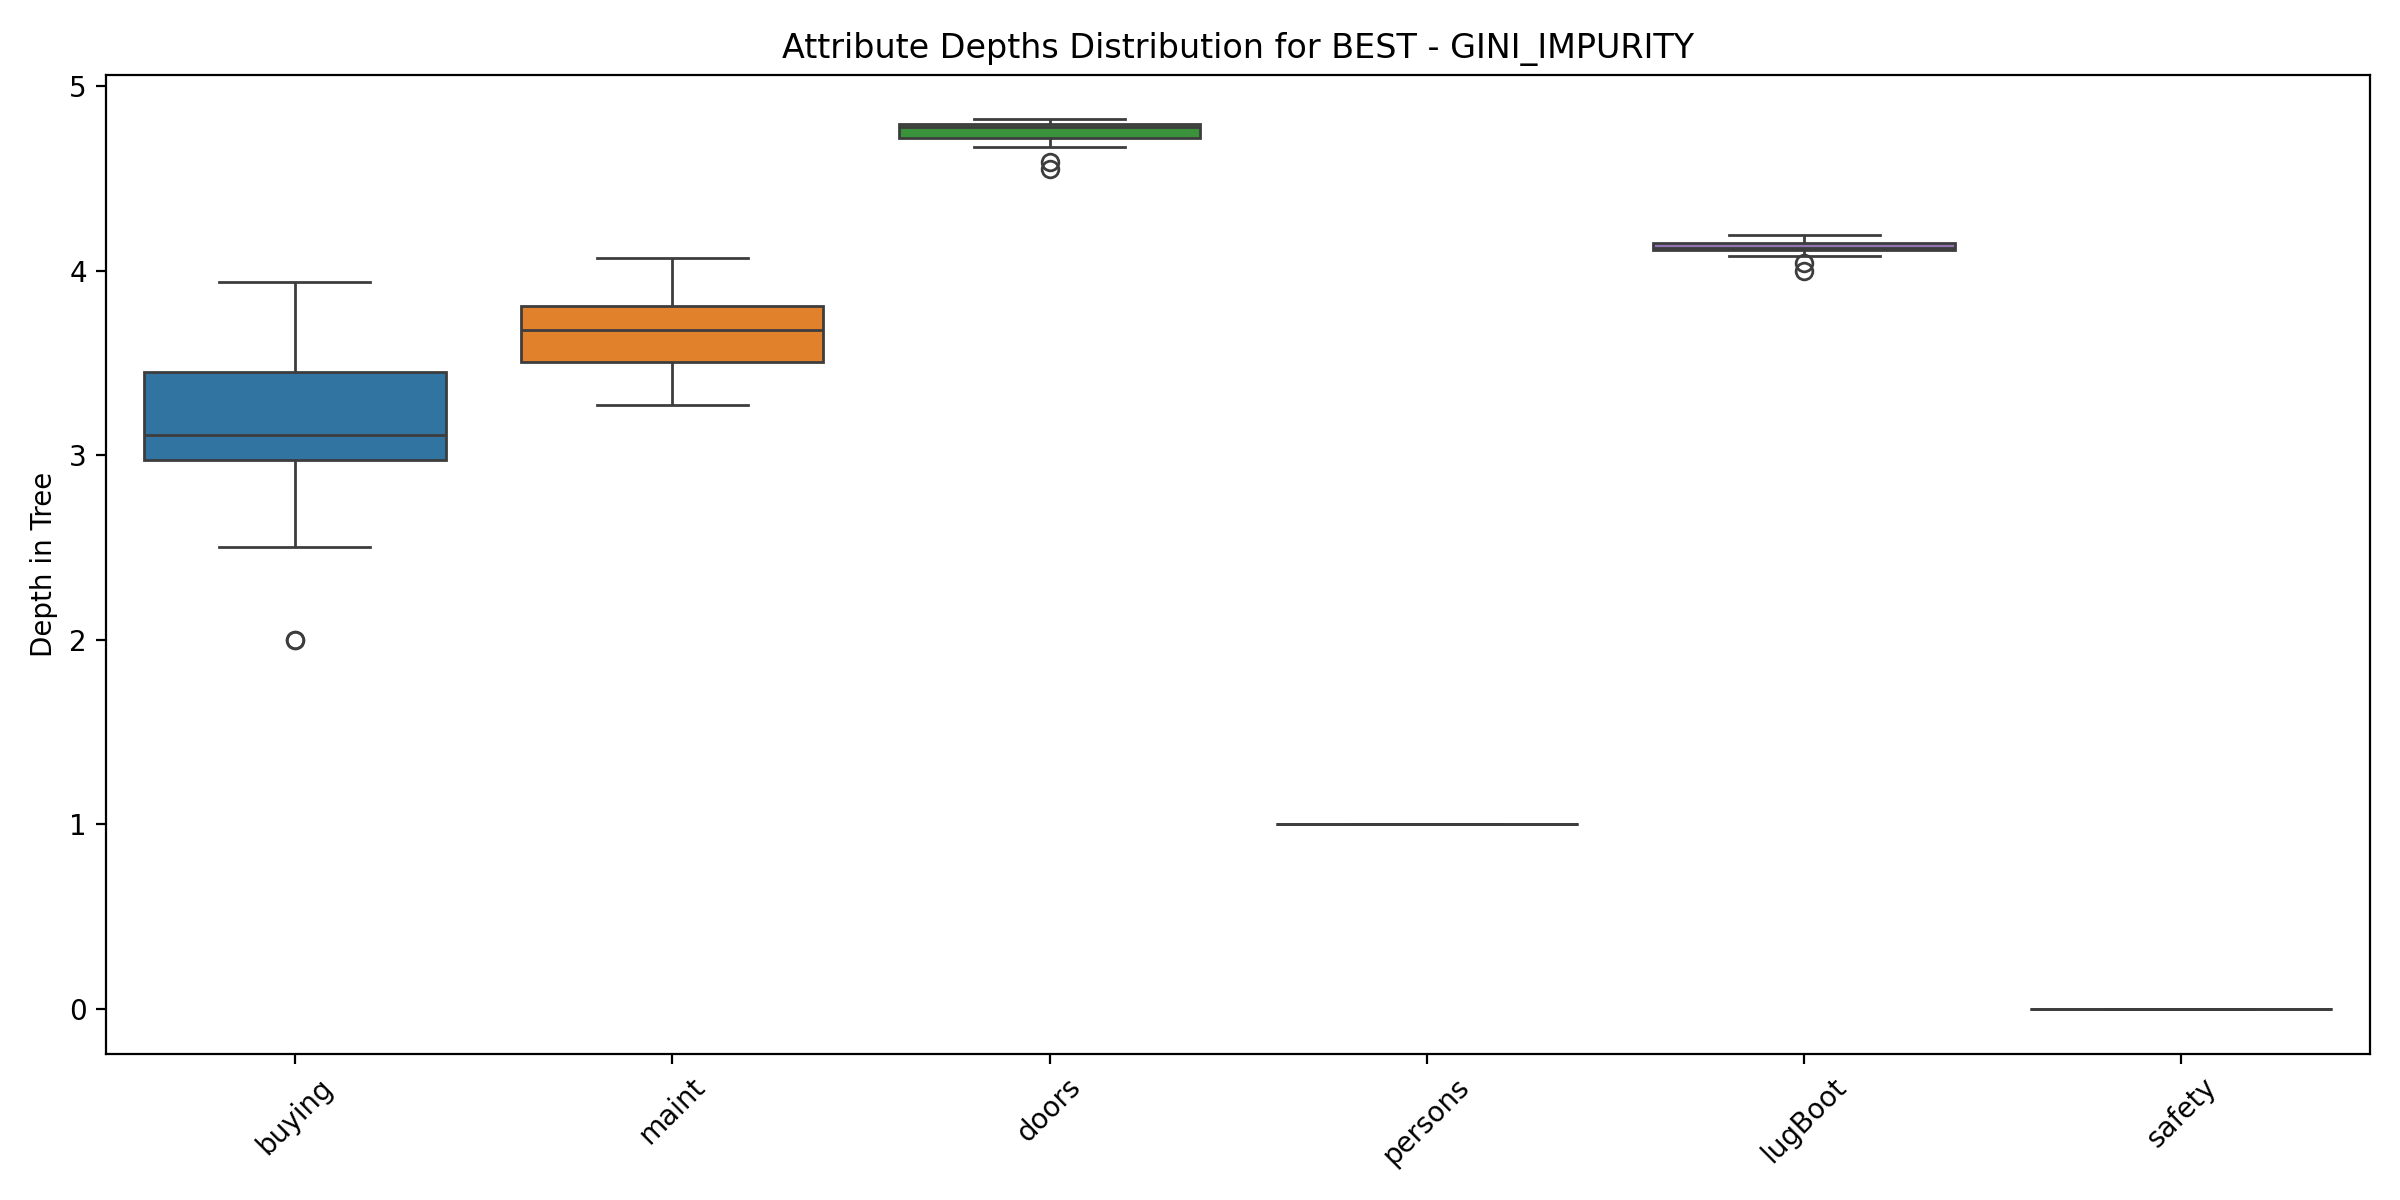
\includegraphics[width=0.9\textwidth]{plots/attribute_depths_BEST_GINI_IMPURITY.png}
    \caption{Distribution of attribute depths for BEST strategy with GINI IMPURITY metric.}
    \label{fig:attr-best-gini}
\end{figure}

This box whisker plot, shows an analysis of the attribute depths. An attribute with lower depth in the tree indicates that it is more crucial in the classification decision. Here, it can be seen that the attributes "safety" and "persons" are the most crucial having depths 0 and 1 consistently in the tree. This means they lie on the topmost decision nodes almost always. Others are placed at higher depths.

\newpage

\begin{figure}[H]
    \centering
    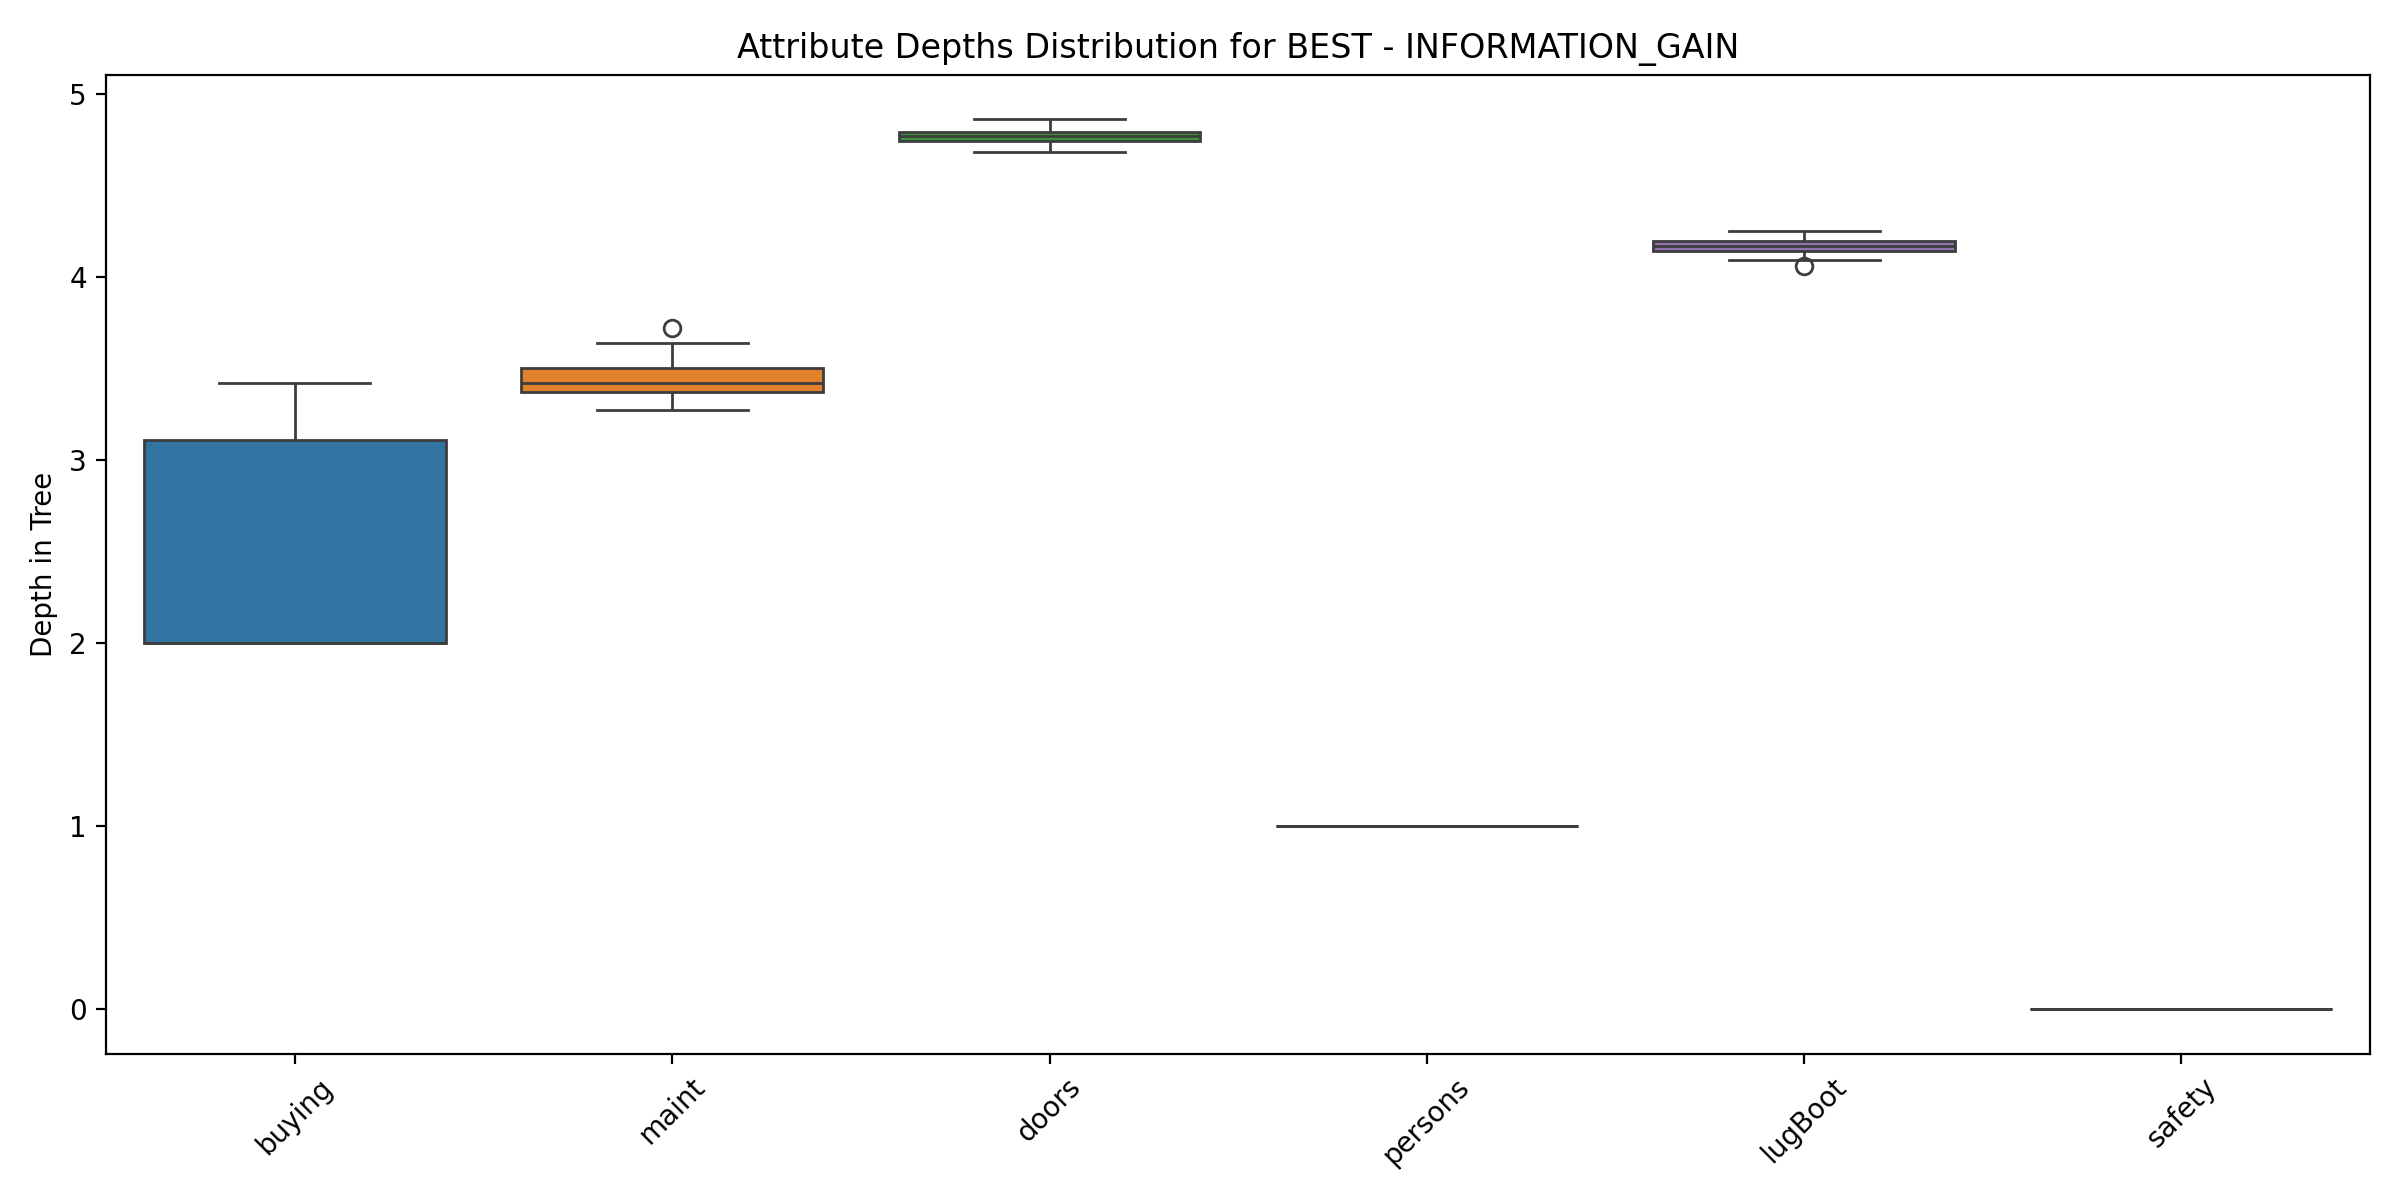
\includegraphics[width=0.9\textwidth]{plots/attribute_depths_BEST_INFORMATION_GAIN.png}
    \caption{Distribution of attribute depths for BEST strategy with INFORMATION GAIN metric.}
    \label{fig:attr-best-ig}
\end{figure}

This plot for the case of Information Gain is very similar to the one above.

\newpage

\begin{figure}[H]
    \centering
    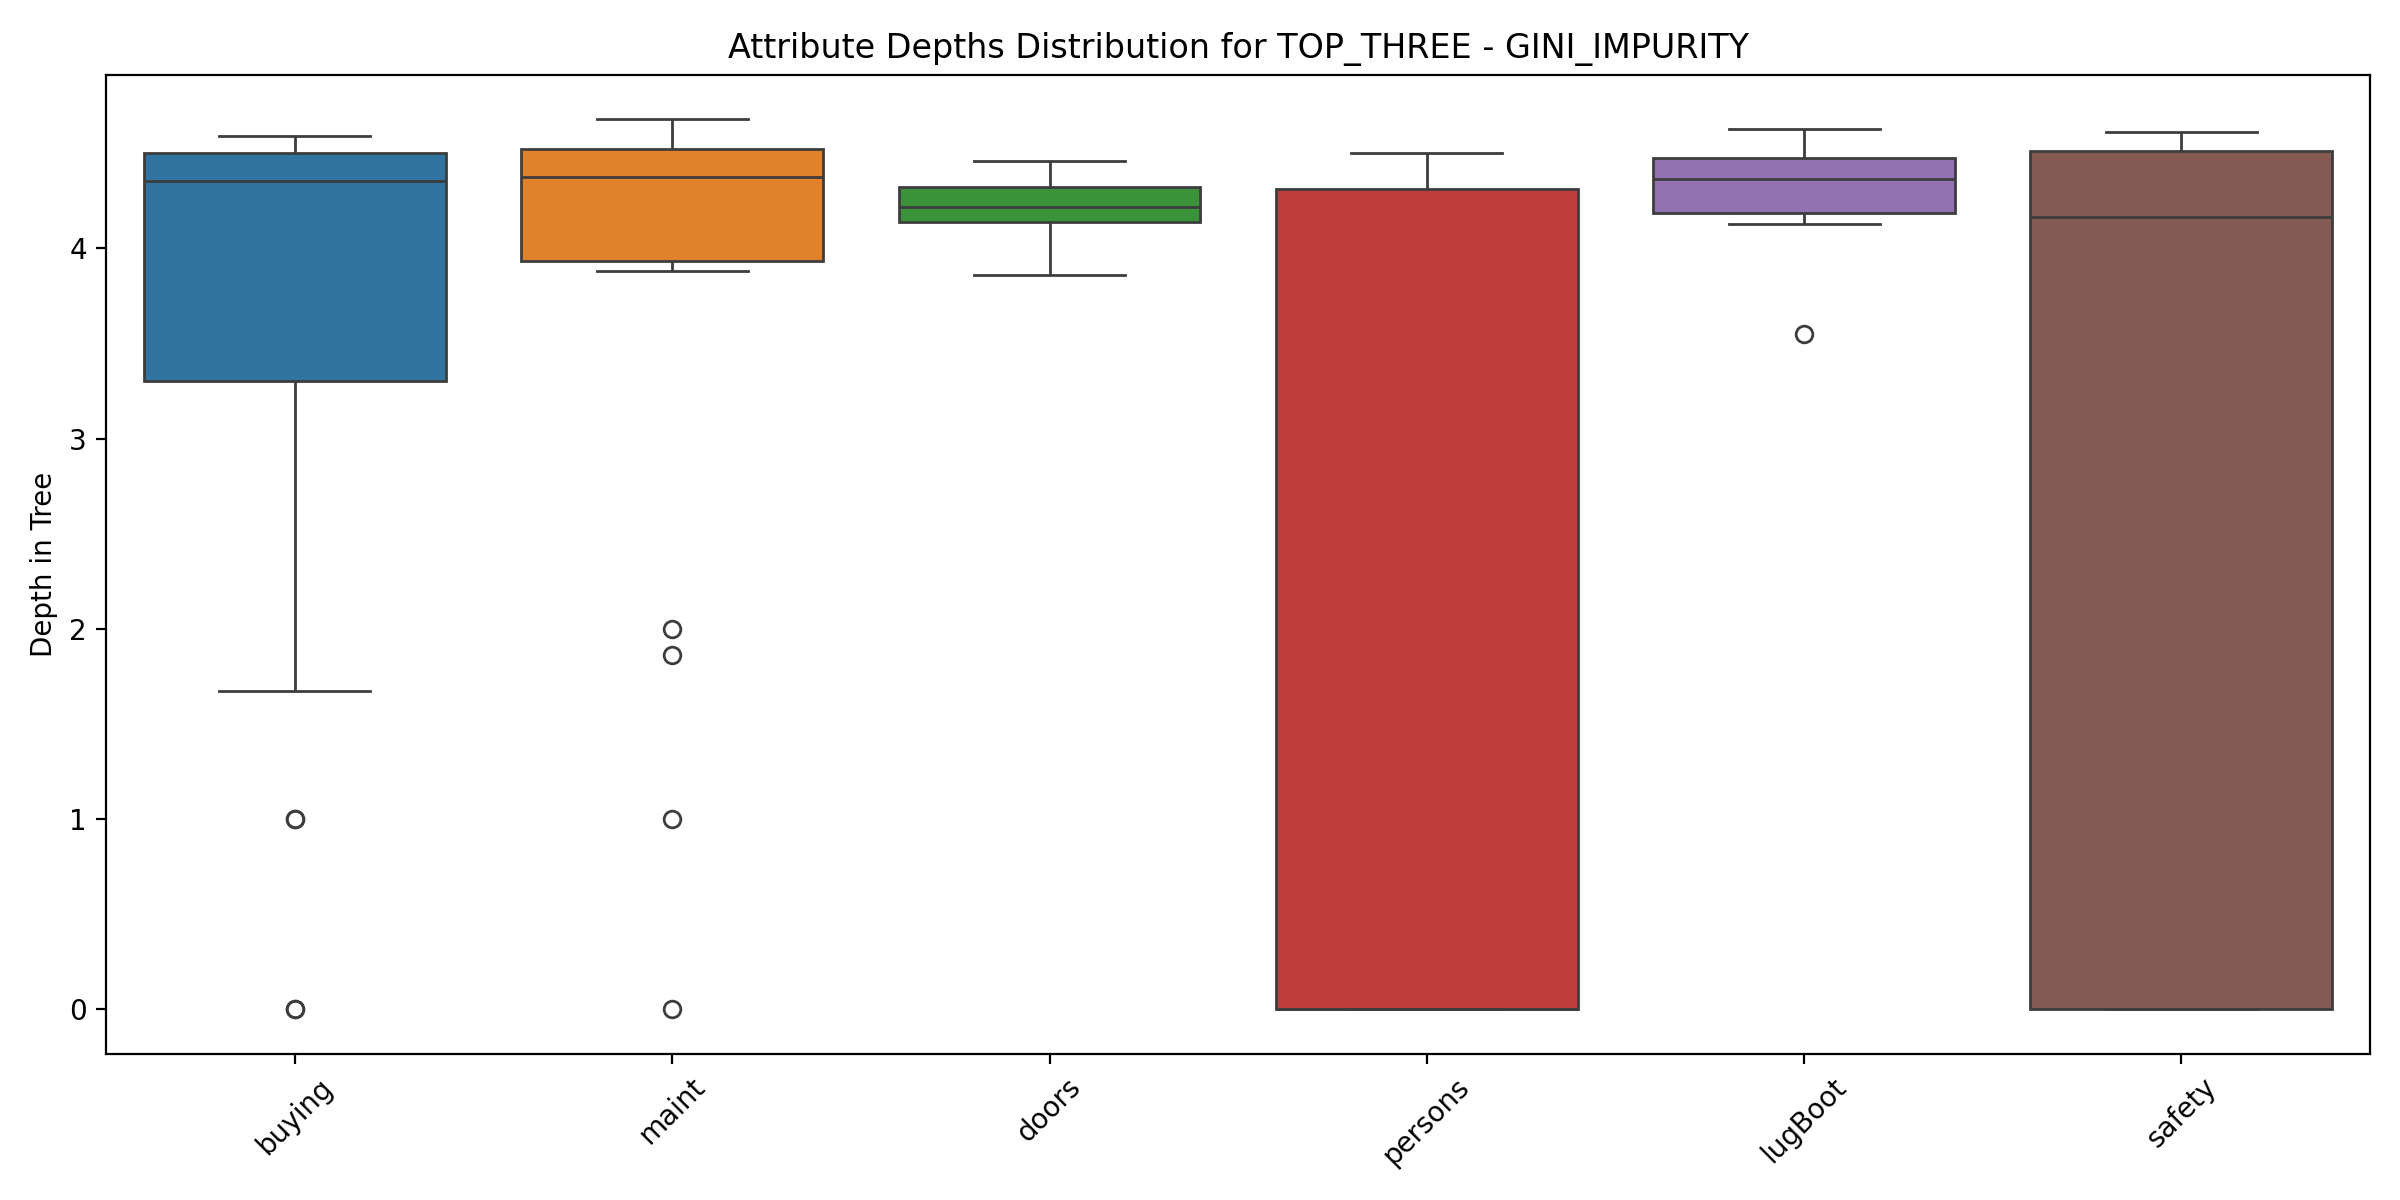
\includegraphics[width=0.9\textwidth]{plots/attribute_depths_TOP_THREE_GINI_IMPURITY.png}
    \caption{Distribution of attribute depths for TOP THREE strategy with GINI IMPURITY metric.}
    \label{fig:attr-top3-gini}
\end{figure}

When we switch the selection strategy, these plots change drastically. The attributes "persons" and "safety" which were always placed closer to the root in the above cases, are now rather being placed at scattered depths ranging from 0 to 5. The reason is that, at the first nodes, due to random choices, often they are rejected. This also explains why the overall accuracy drops significantly in case of random choice.

\newpage

\begin{figure}[H]
    \centering
    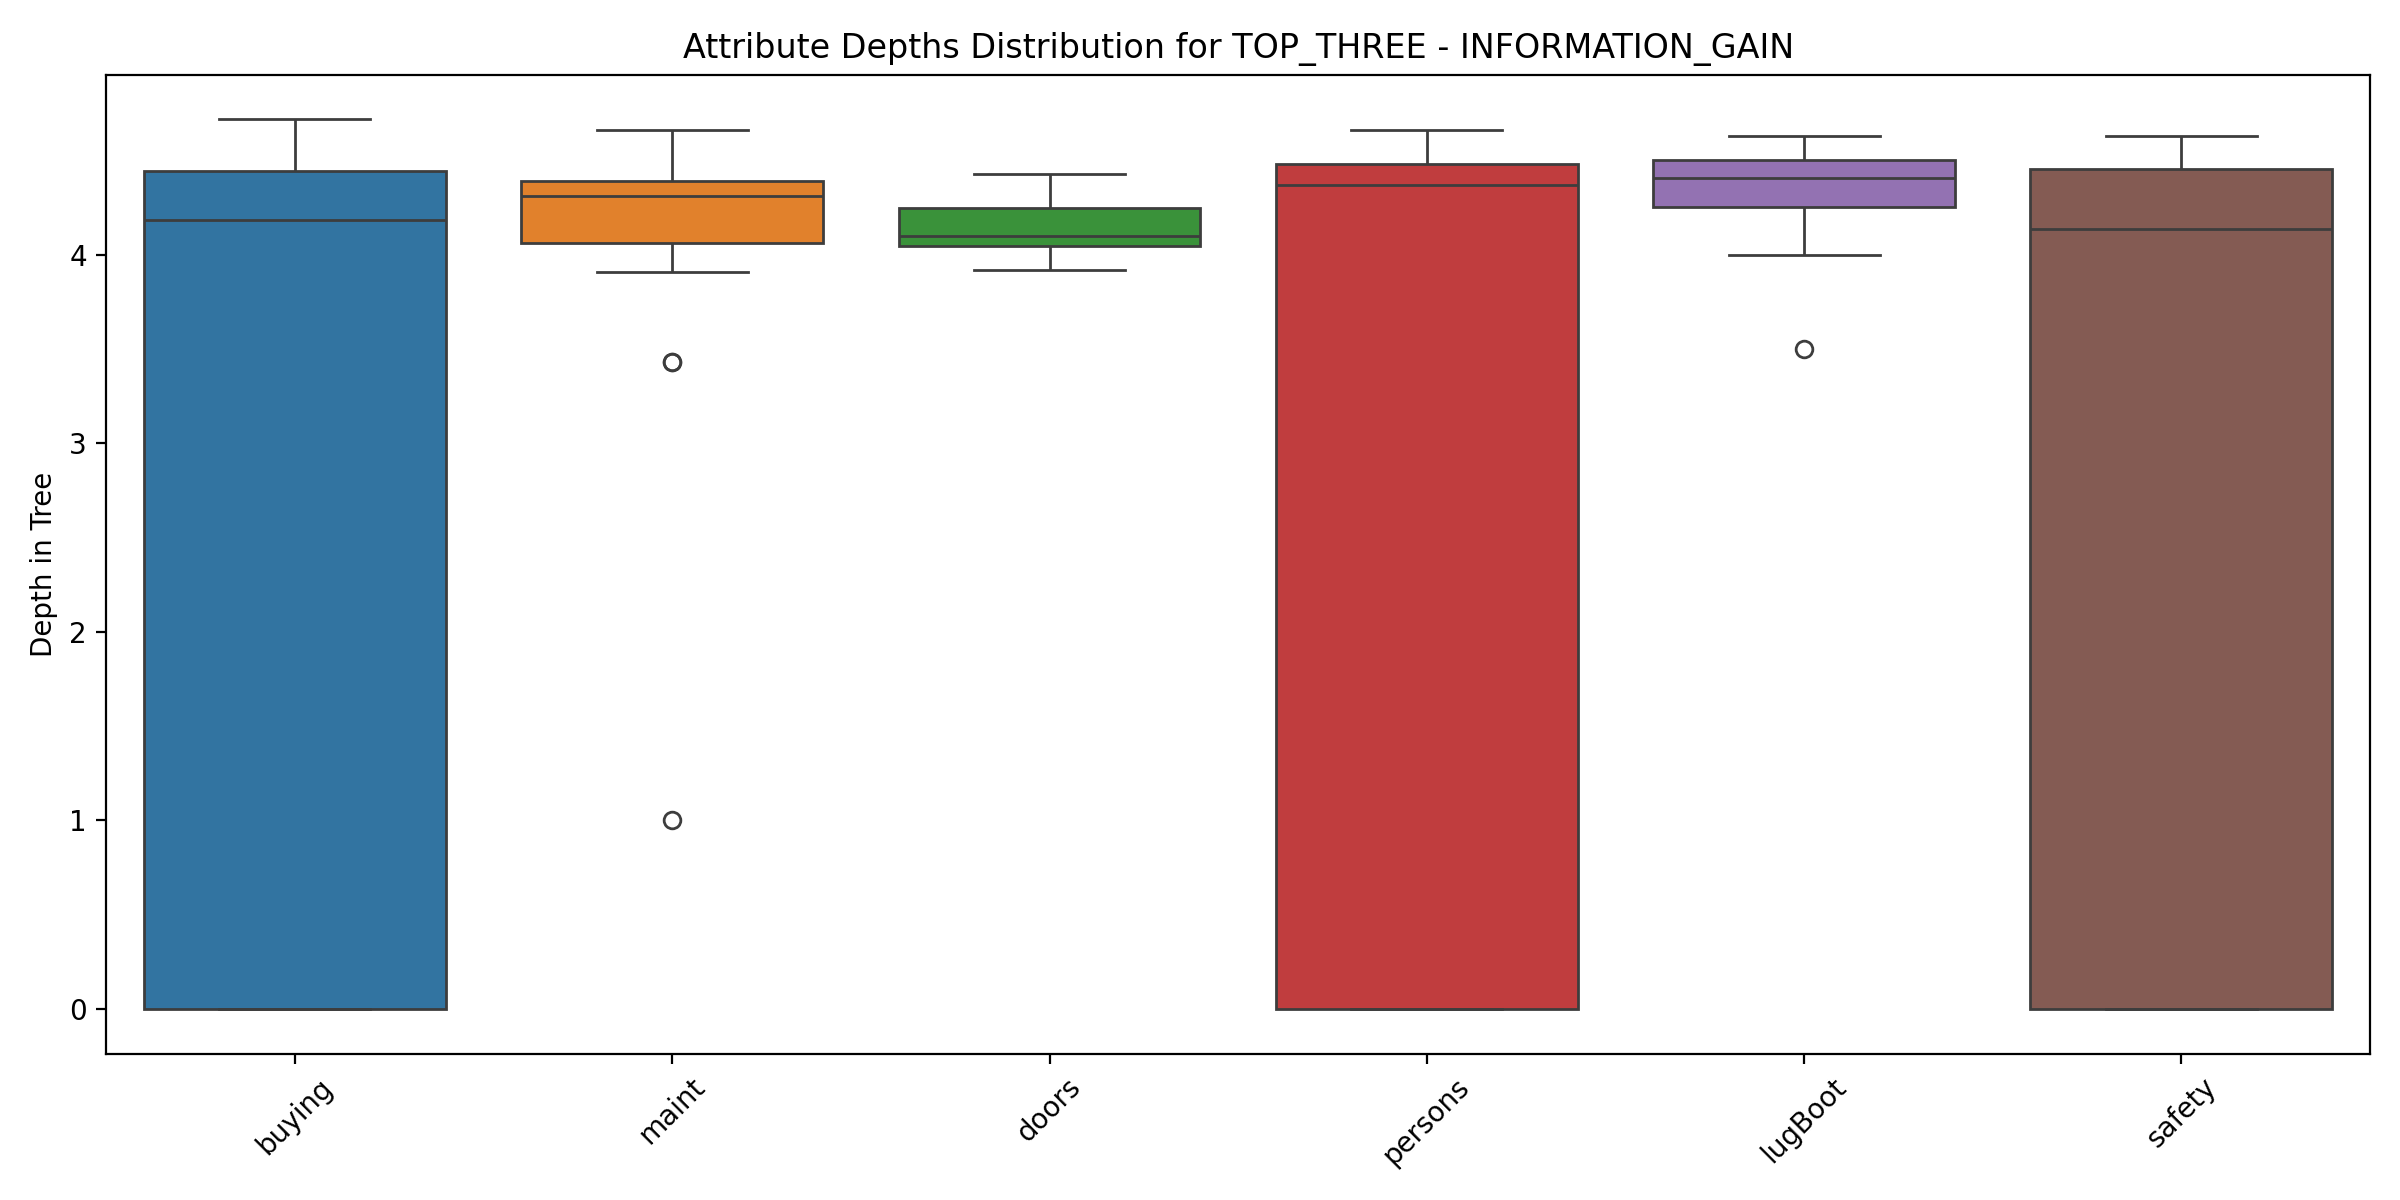
\includegraphics[width=0.9\textwidth]{plots/attribute_depths_TOP_THREE_INFORMATION_GAIN.png}
    \caption{Distribution of attribute depths for TOP THREE strategy with INFORMATION GAIN metric.}
    \label{fig:attr-top3-ig}
\end{figure}

This plot for the case of Information Gain is very similar to the one above.

\newpage

% Training Metrics (Individual plots)
\subsection{Training Metrics Analysis}

\begin{figure}[H]
    \centering
    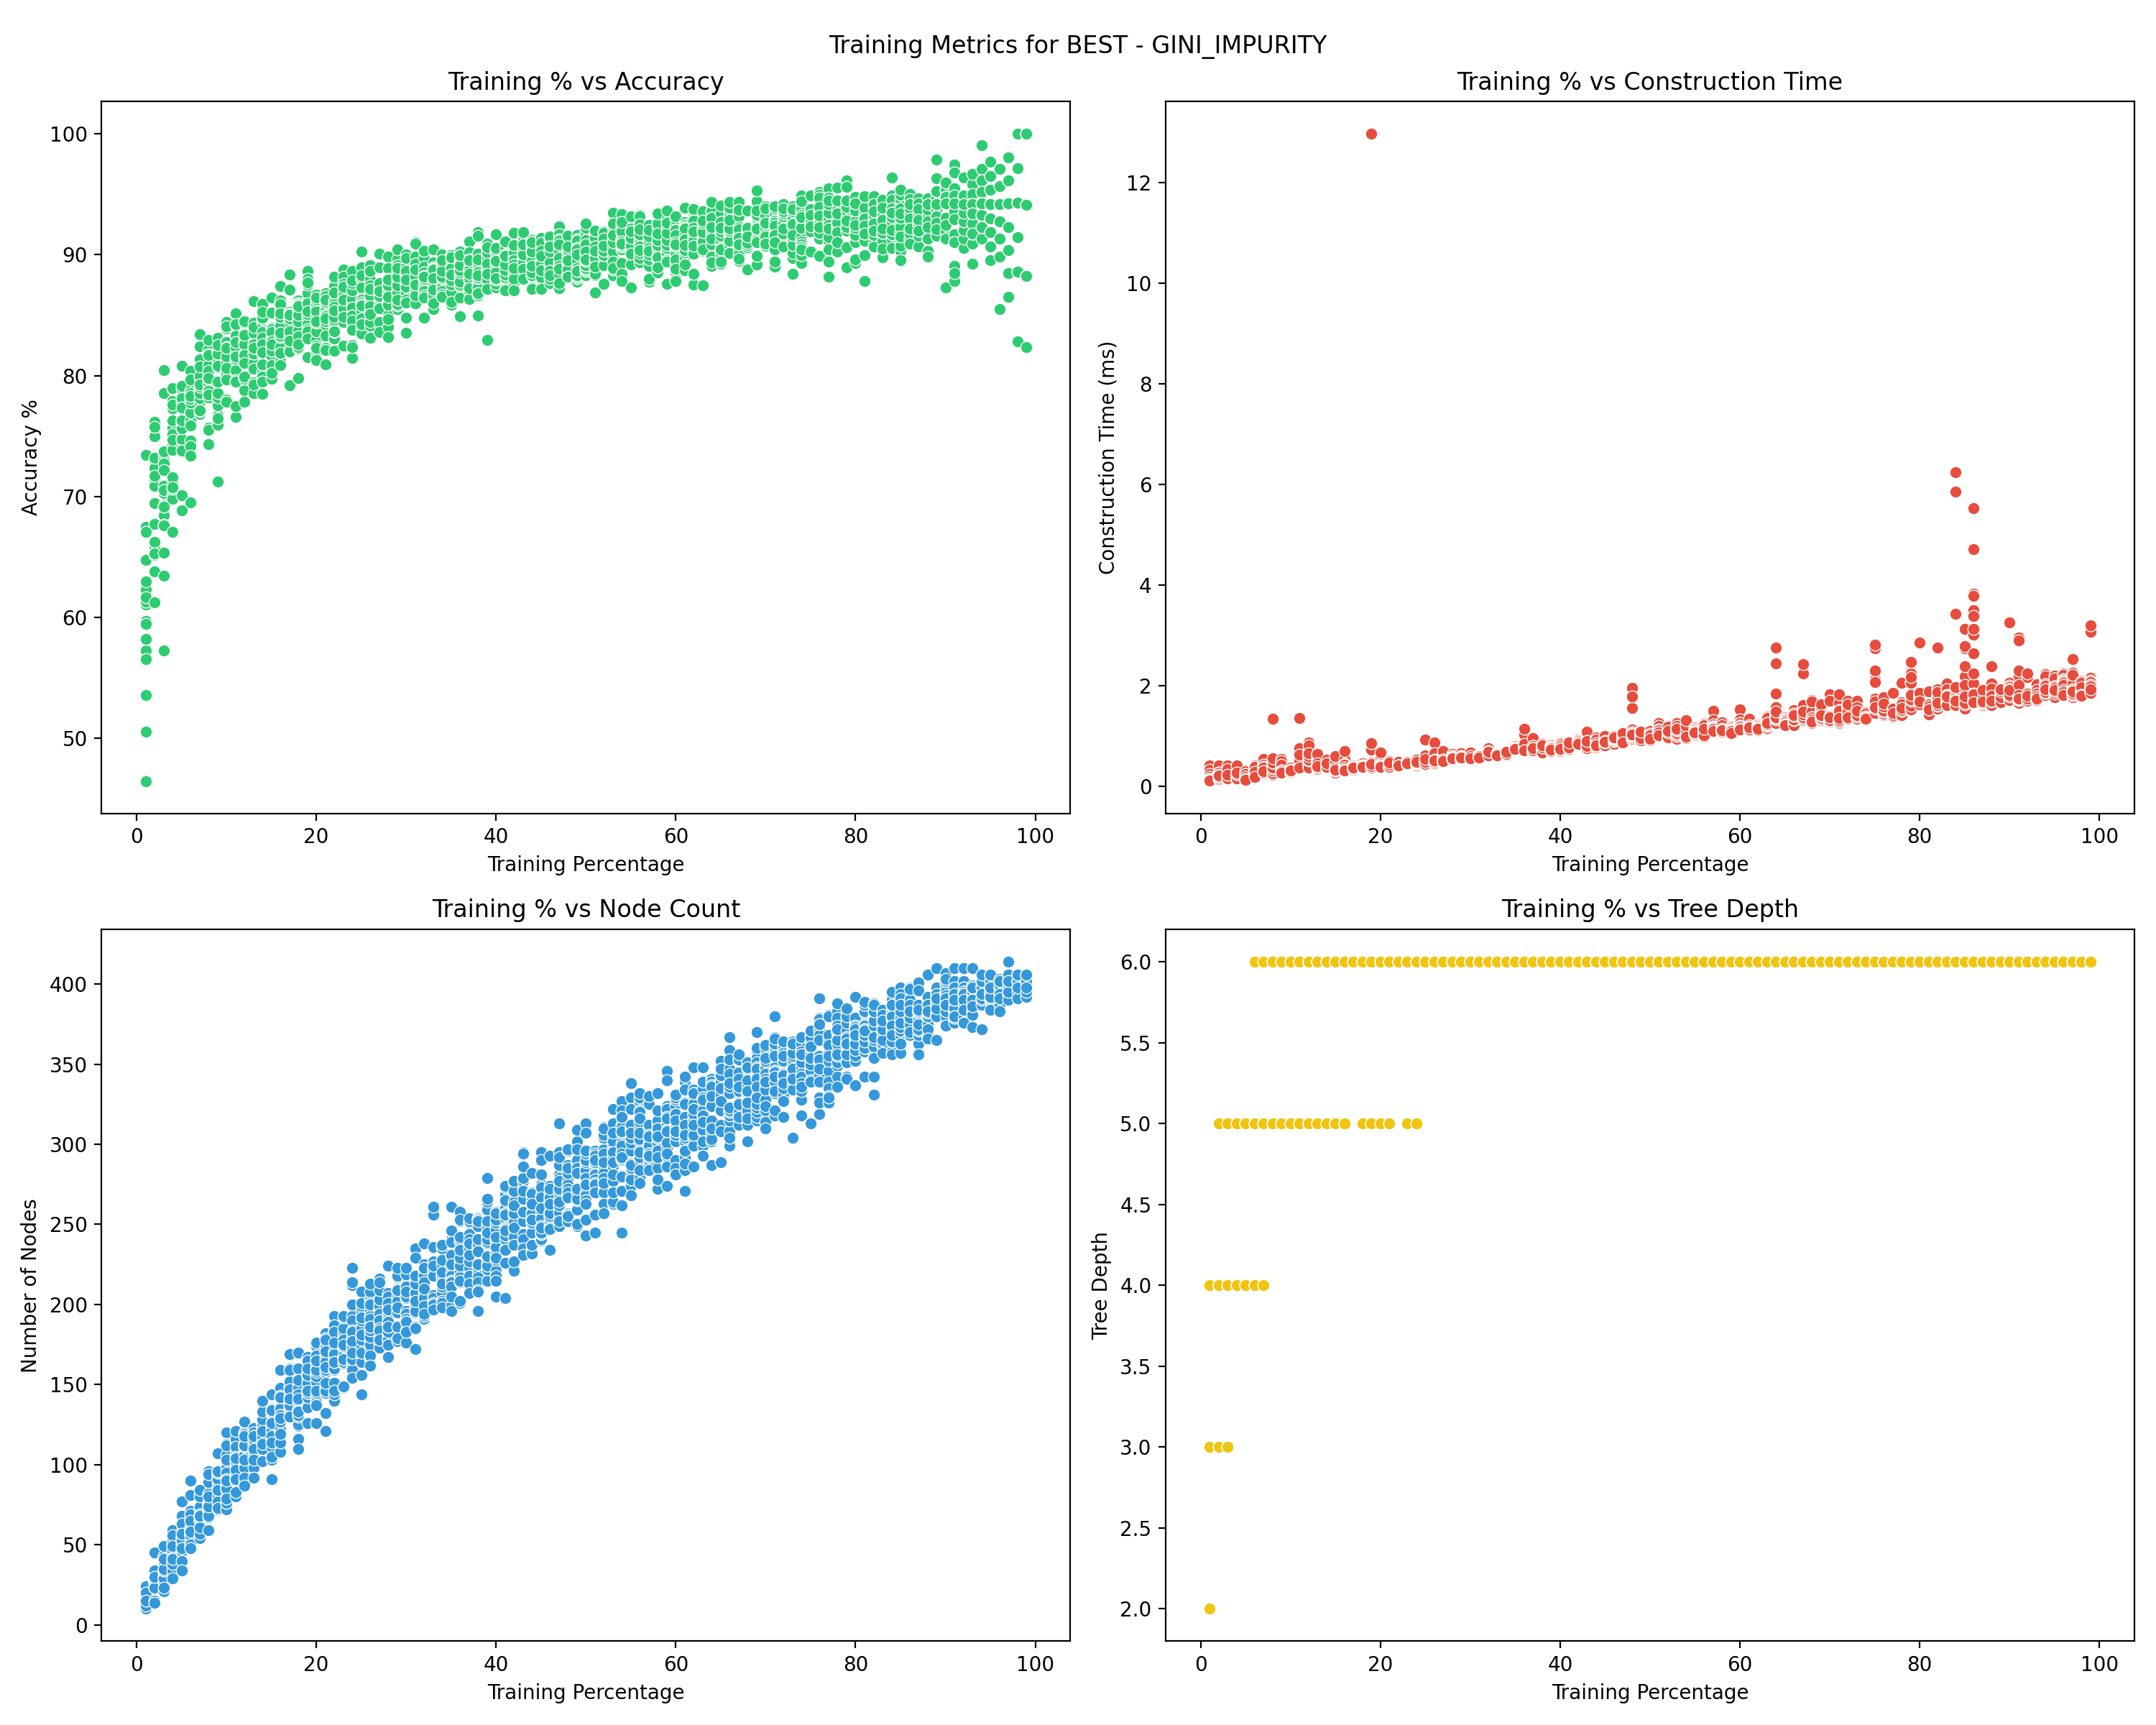
\includegraphics[width=0.9\textwidth]{plots/training_metrics_BEST_GINI_IMPURITY.png}
    \caption{Training metrics for BEST strategy with GINI IMPURITY metric showing relationships between training percentage and various performance measures.}
    \label{fig:training-best-gini}
\end{figure}
\newpage

\begin{figure}[H]
    \centering
    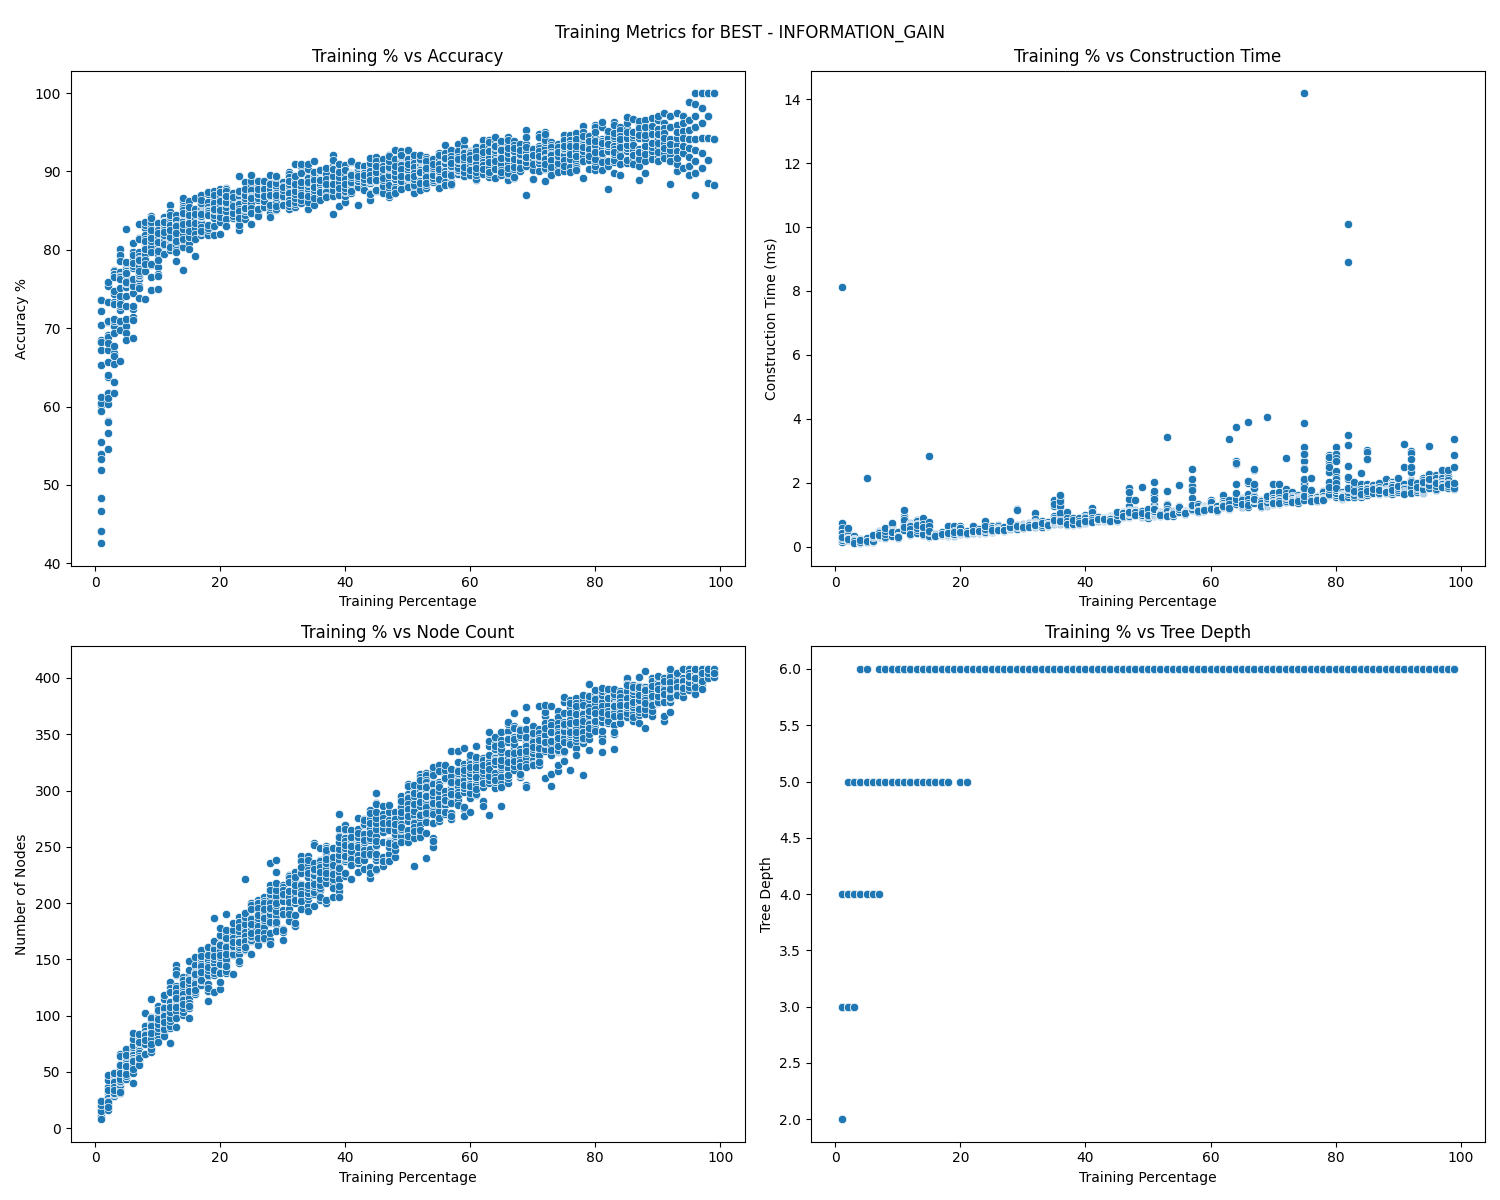
\includegraphics[width=0.9\textwidth]{plots/training_metrics_BEST_INFORMATION_GAIN.png}
    \caption{Training metrics for BEST strategy with INFORMATION GAIN metric showing relationships between training percentage and various performance measures.}
    \label{fig:training-best-ig}
\end{figure}
\newpage

\begin{figure}[H]
    \centering
    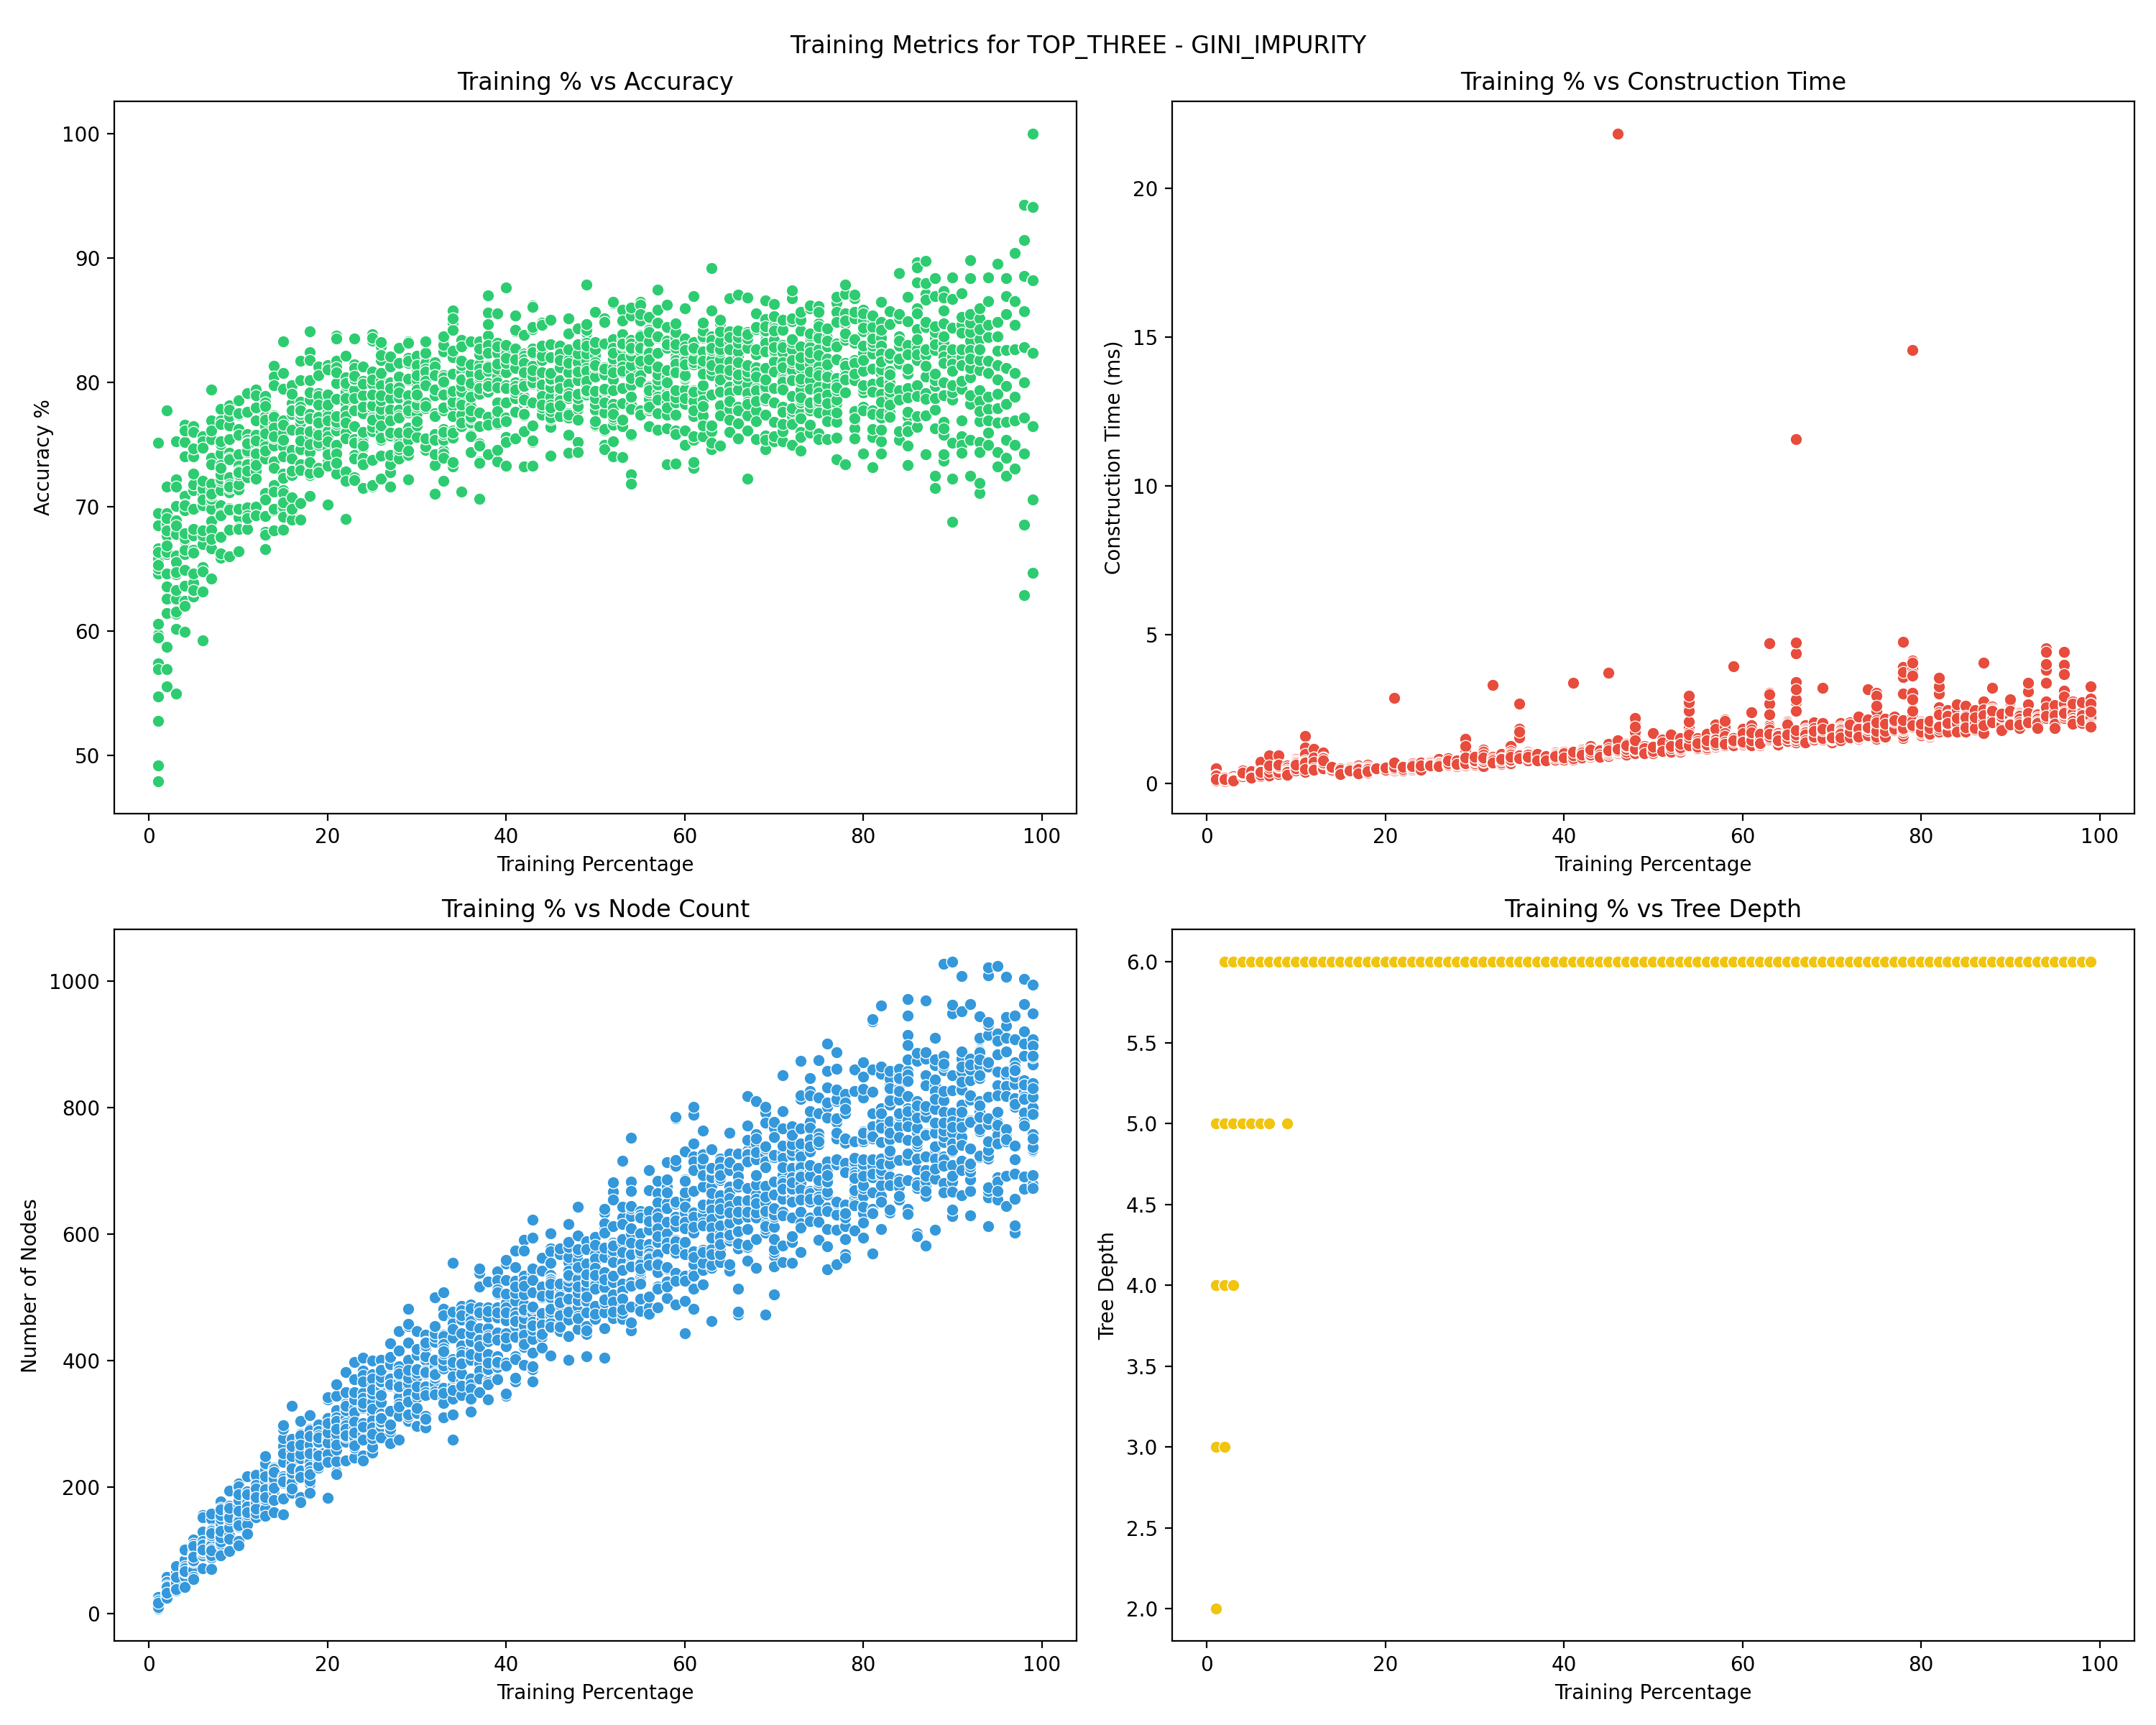
\includegraphics[width=0.9\textwidth]{plots/training_metrics_TOP_THREE_GINI_IMPURITY.png}
    \caption{Training metrics for TOP THREE strategy with GINI IMPURITY metric showing relationships between training percentage and various performance measures.}
    \label{fig:training-top3-gini}
\end{figure}
\newpage

\begin{figure}[H]
    \centering
    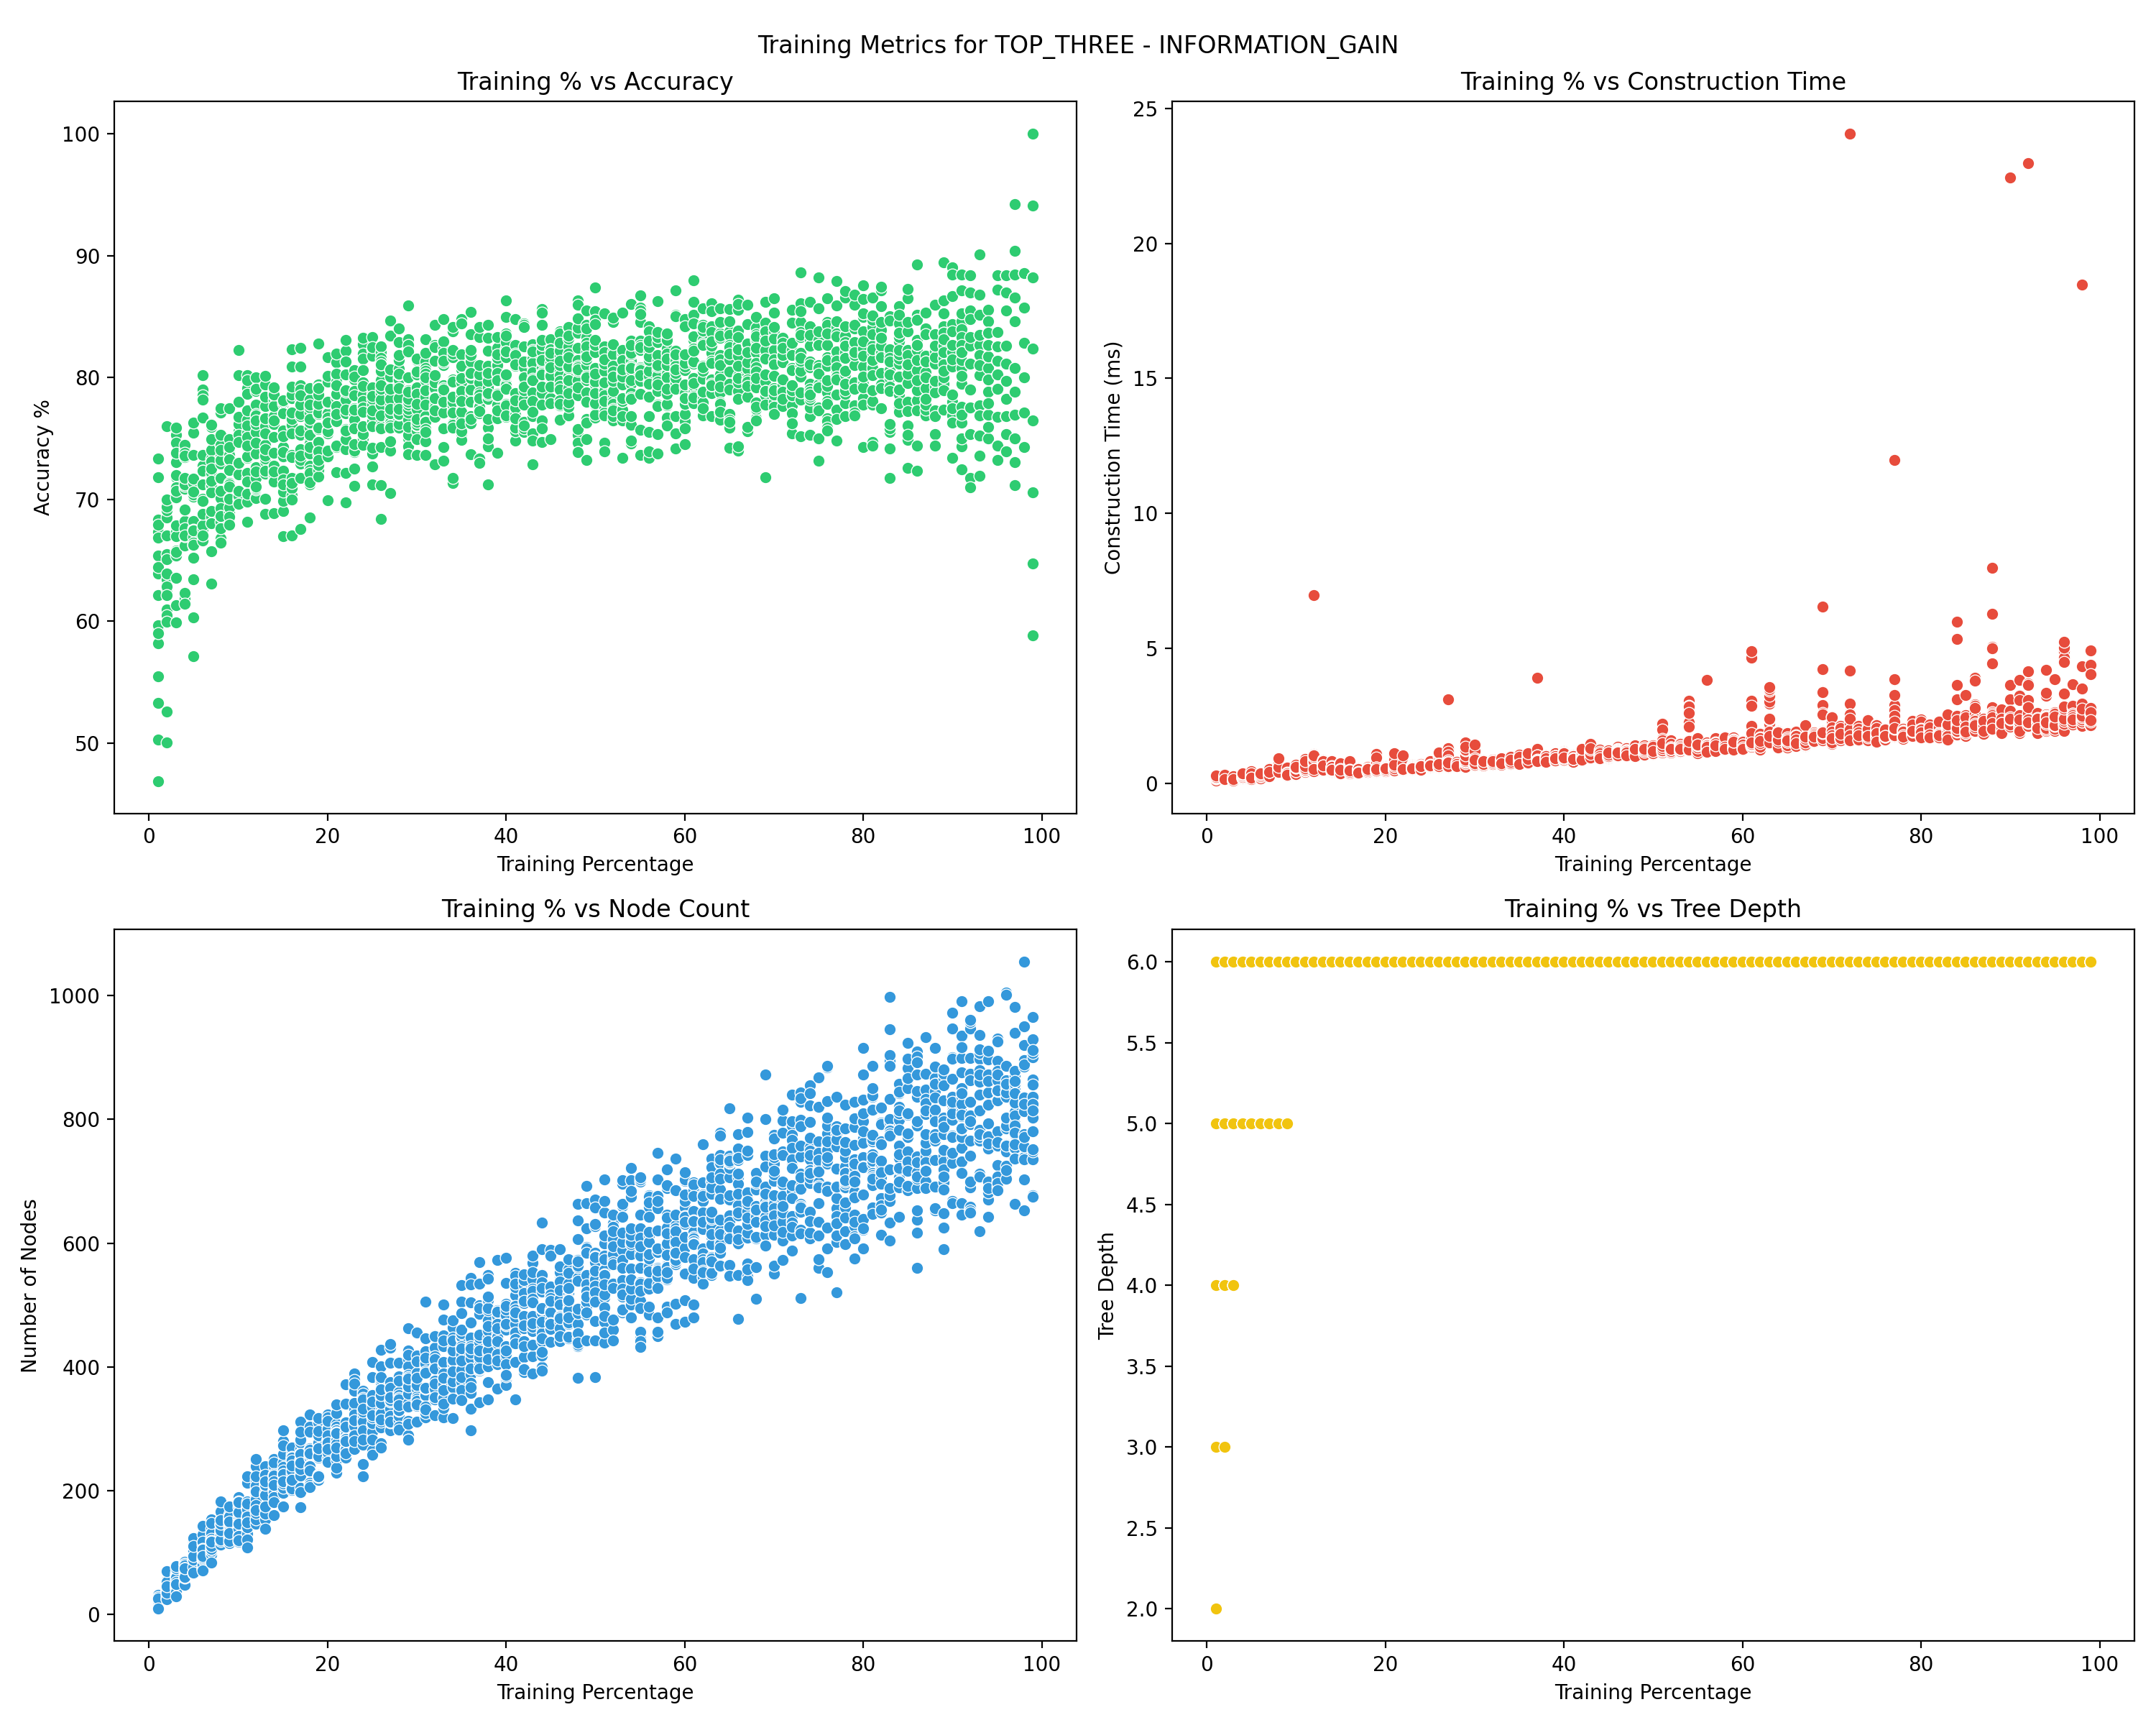
\includegraphics[width=0.9\textwidth]{plots/training_metrics_TOP_THREE_INFORMATION_GAIN.png}
    \caption{Training metrics for TOP THREE strategy with INFORMATION GAIN metric showing relationships between training percentage and various performance measures.}
    \label{fig:training-top3-ig}
\end{figure}

\end{document}
